\cotefile{136}
\scanpage{142}
\mspage{2}
\begin{center}- 134 -\end{center}
\margin{IX}

et, en vertu de la structure connue de $I$ ($I\qquad$), une suite exacte
\[
(11.3.3)\qquad 1\longrightarrow R\longrightarrow I\longrightarrow T\longrightarrow 1\quad,
\]
avec $R$ un groupe pro-fini \uline{premier à $\ell$}. Si maintenant nous \uline{partons} de données (11.3.2) et (11.3.3), et introduisons les groupes
\[
(11.3.4)\qquad \Phi=(U\otimes D_\ell)^I/U^I\otimes D_\ell\ ,\quad
\Phi'=(U'\otimes D_\ell)^I/U'^I\otimes D_\ell\ ,\quad
(D_\ell=\mathbb{Q}_\ell/\mathbb{Z}_\ell)
\]
nous allons définir une dualité parfaite
\[
(11.3.5)\qquad \Phi\otimes\Phi'\longrightarrow\mathbb{Q}/\mathbb{Z}\quad,
\]
ce qui nous donnera en particulier l'accouplement annoncé (11.3.1).
Considérons la suite exacte de $I$-modules
\[
(11.3.6)\qquad 0\longrightarrow U\xrightarrow{i}U\otimes_{\mathbb{Z}_\ell}\mathbb{Q}_\ell
\xrightarrow{j}U\otimes D_\ell\longrightarrow 0\quad,
\]
et la suite exacte de cohomologie associée, en prenant la cohomologie de $I$ définie par les \uline{cochaînes continues} à coefficients dans les groupes topologiques envisagés :
\diagram{
\begin{tikzcd}[column sep=small]
(11.3.7) & 0 \arrow[r] & H^{\unsure{o|0}}(I,U) \arrow[r,"i^{\unsure{o|0}}"] \arrow[d,phantom,"\wr" description] & H^{\unsure{o|0}}(I,U\otimes\mathbb{Q}_\ell) \arrow[r,"j^{\unsure{o|0}}"] \arrow[d,phantom,"\wr" description] & H^{\unsure{o|0}}(I,U\otimes D_\ell) \arrow[r,"\partial"] \arrow[d,phantom,"\wr" description] & H^1(I,U) \arrow[r,"i^1"] & H^1(I,U\otimes\mathbb{Q}_\ell) \arrow[d,phantom,"\wr" description] \\
& & U^I & (U\otimes\mathbb{Q}_\ell)^I\simeq U^I\otimes_{\mathbb{Z}}\mathbb{Q} & (U\otimes D_\ell)^I & & H^1(I,U)\otimes_{\mathbb{Z}}\mathbb{Q}\ .
\end{tikzcd}
}
Il est immédiat que $\Phi$ défini par (11.3.4) n'est autre que $\operatorname{coker}j^{\unsure{o|0}}$, donc est canoniquement isomorphe à $\operatorname{Ker}i^1$, i.e. on trouve une suite exacte canonique
\[
(11.3.8)\qquad 0\longrightarrow\Phi\longrightarrow H^1(I,U)\longrightarrow H^1(I,U)\otimes_{\mathbb{Z}}\mathbb{Q}\quad,
\]
\margin{452}
\margin{452}
\margin{\unsure{141}}
\scanpage{143}
\begin{tabular}{llllllll}
\unsure{12.24.16} & \unsure{P} & 16 AUG 82 & \unsure{R6.PR1} & SYS JES2 & JOB 224 & END & A****\\
\unsure{12.24.21} & \unsure{P} & 16 AUG 82 & \unsure{R6.PR1} & SYS JES2 & JOB 224 & END & A****\\
\unsure{12.23.21} & \unsure{P} & 16 AUG 82 & \unsure{R6.PR1} & SYS JES2 & JOB 224 & END & A****\\
\unsure{12.23.21} & \unsure{P} & 16 AUG 82 & R6.PR1 & SYS JES2 & JOB 224 & END & A****\\
\unsure{12.23.11} & \unsure{P} & 16 AUG 82 & R6.PR1 & SYS JES2 & JOB 224 & END & A****\\
\unsure{12.23.10} & \unsure{P} & 16 AUG 82 & \unsure{R6.PR1} & SYS JES2 & JOB \unsure{224} & \unsure{END} & \unsure{A****}
\end{tabular}

\diagram{
\[
\begin{array}{lll}
\texttt{\unsure{AA}} & \texttt{YY}\hspace{8em}\texttt{YY} & \texttt{\unsure{22222222222}}\\
\texttt{\unsure{AA}} & \texttt{YY}\hspace{8em}\texttt{YY} & \texttt{\unsure{22222222222}}\\
\texttt{\unsure{AA}} & \hspace{1em}\texttt{YY}\hspace{6em}\texttt{YY} & \hspace{10em}\texttt{22}\\
\texttt{AA} & \hspace{2em}\texttt{YY}\hspace{4em}\texttt{YY} & \hspace{10em}\texttt{22}\\
\texttt{AA} & \hspace{3em}\texttt{YY}\hspace{2em}\texttt{YY} & \hspace{10em}\texttt{22}\\
\texttt{\unsure{AAAA}} & \hspace{4em}\texttt{YYYY} & \hspace{8em}\texttt{\unsure{22}}\\
\texttt{\unsure{AAAA}} & \hspace{5em}\texttt{YY} & \hspace{6em}\texttt{\unsure{22}}\\
\texttt{AA} & \hspace{5em}\texttt{YY} & \hspace{4em}\texttt{22}\\
\texttt{AA} & \hspace{5em}\texttt{YY} & \hspace{2em}\texttt{22}\\
\texttt{AA} & \hspace{5em}\texttt{YY} & \texttt{22}\\
\texttt{\unsure{AA}} & \hspace{5em}\texttt{YY} & \texttt{\unsure{22222222222}}\\
\texttt{\unsure{AA}} & \hspace{5em}\texttt{YY} & \texttt{\unsure{2222222222}}
\end{array}
\]
}
\margin{142}
\scanpage{144}
\figure{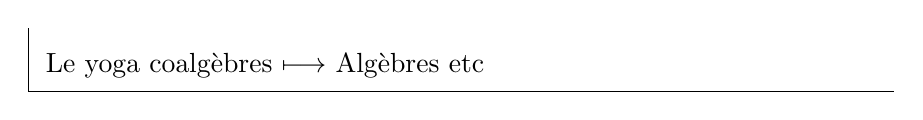
\begin{tikzpicture}\node[anchor=south west] at (0.1,0.05) {Le yoga coalgèbres $\longmapsto$ Algèbres \unsure{etc}};\draw (0,0.8)--(0,0)--(11,0);\end{tikzpicture}}

$\unsure{k}$ anneau, on travaille dans le topos $\widehat C$, où $C_k$ est la catégorie des $k$-algèbres. Le foncteur oubli
\[
C_k\longrightarrow\mathrm{Ens}\qquad A\longmapsto A
\]
est un \deleted{\unsure{faisceau|foncteur} vers les Algèbres}\inserted{objet de $\widehat C_k$ muni d'une structure} de $k$-Algèbre, appelé $O_k$. Si $M$ est un $k$-module, $V(M)$ (\unsure{ou} $V_k(M)$ au besoin) est le \deleted{\unsure{faisceau|foncteur}} $O_k$-Module
\[
V(M)_{\deleted{\unsure{k}}}(\unsure{A})=\operatorname{Hom}_{k\text{-mod}}(M,A)=\operatorname{Hom}_{A\text{-mod}}(M_A,A)
\]
$V(M)$ dépend fonctoriellement de $M$, de façon contravariante, et on voit que $V$ est un foncteur \uline{pl. fd.} des $k$-modules vers les $O_k$-Modules
\[
\operatorname{Hom}_k(M,N)\xrightarrow{\sim}\operatorname{Hom}_{O_k}(V(N),V(M))
\]
\inserted{comme $V(\unsure{N|M})$ est repr. par $\operatorname{Sym}^*(N)$,} De façon générale, un morphisme dans $\widehat C_k$
\[
V(N)\longrightarrow\deleted{V(M)=\operatorname{Spec}(B)}F\qquad(\text{si }F\in\mathrm{ob}\widehat C_k)
\]
\deleted{\unsure{et}} correspond à un \deleted{hom dans $C_k$} élément de $F(\deleted{\unsure{B}}\operatorname{Sym}^*(N))$
\[
\operatorname{Hom}_{\widehat C_k}(V(N),F)\simeq F(\operatorname{Sym}^*(N))
\]
en particulier si $F=\operatorname{Spec} B$
\[
\operatorname{Hom}_{\widehat C_k}(V(N),\operatorname{Spec}B)\simeq
\operatorname{Hom}_{k\text{-alg}}(B,\operatorname{Sym}^*(N))
\]
et faisant $B=\operatorname{Sym}^*(M)$ il vient
\[
\operatorname{Hom}_{\widehat C_k}(V(N),V(M))\simeq
\operatorname{Hom}_{k\text{-mod}}(M,\operatorname{Sym}^*N)
\]
Soit
\[
u^*:V(N)\mathbin{\text{---}}V(M)
\]
correspondant à
\[
u:M\longrightarrow\operatorname{Sym}^*(N).
\]
On \unsure{convient|constate} que
\[
\deleted{\unsure{\lambda^2\longmapsto u(\lambda)}}
\qquad u(m)=\sum u_i(m)\qquad u_i(m)\in\operatorname{Sym}^i(N)
\]
(la famille des \deleted{$\unsure{u_i:M}$} \deleted{\unsure{est} ``loc. finie''}
\[
u_i:M\mathbin{\text{---}}\operatorname{Sym}^i(N)
\]
``loc. finie''), alors on a pour $\lambda\in\unsure{O_k}(A)=A$
\margin{143}
\scanpage{145}
et $x^*\in V(N)(A)=\operatorname{Hom}_{k\text{-mod}}(N,A)$,
\diagram{
\begin{tikzcd}
u^*(x^*)=\widetilde{x}^*\circ u & M\arrow[r,"u"] & \operatorname{Sym}^*N\arrow[r,"\widetilde{x}^*"] & A\\
\operatorname{Hom}_{k\text{-mod}}(M,A)\arrow[u,phantom,"\in" description,sloped] & & &
\end{tikzcd}
}
où $\widetilde{x}^*$ est l'hom de $k$-Alg. \unsure{prolgt} can. de $x^*$.

On a donc
\[
u^*(x^*)(\deleted{\unsure{x}}\inserted{m})=
\sum_{i\geq0}\widetilde{x}^{*i}(u_i(\unsure{x|m}))
\qquad(\widetilde{x}^{*i}\text{ étant la }\deleted{\unsure{exten-}}\inserted{restr.}\text{ de }x^*\text{ à }\operatorname{Sym}^iN)
\]
d'où, si $\lambda\in A$
\[
u^*(\lambda x^*)(m)=\sum_{i\geq0}\lambda^i\widetilde{x}^{*i}(u_i(m))
=\sum_{i\geq0}(\deleted{\unsure{\lambda^i}}\widetilde{x}^{*i})\unsure{((\lambda^iu_i)m)}
\]
Donc dans la correspondance entre $u^*$ et $u$, sur $k$ ou après chgt. de base sur un $A$, la \deleted{multiplication}\inserted{composition} \deleted{\unsure{par $u$}} de $x^*$ avec une homothétie \deleted{$\unsure{\lambda(N_A)=\lambda\in A}$} $\lambda$ dans le $O_k$-module $N$ (ou $O_A$-module $N_A$) correspond à l'opération
\[
u=\sum u_i\longmapsto u^\lambda=\sum\lambda^iu_i.
\]
On en conclut que $u^*$ est \uline{homogène de} degré $n$ (i.e. satisfait, pour $A$, $\lambda$ variables,
\[
:\quad u^*\circ\lambda_{V(N)}=\lambda^n_{V(M)}\circ u^*
\]
ssi tous les $u_i$ pour $i\neq n$ sont nuls, i.e. ssi $u$ est un hom
\[
M\mathbin{\text{---}}\operatorname{Sym}^nN.
\]
[En effet, il faut avoir $\sum(\lambda^i-\lambda^n)u_i=0$ $\forall A,\lambda\in A$, prenant $A=k[T]$ et $\lambda=T$, on doit avoir
\[
\sum_{i\neq n}(T^i-T^n)u_i\unsure{(x)}=0\ ,\quad
\text{i.e. }\sum(T^i-T^n)u_i(x)=0
\]
pour tt $x\in M$, $n\neq i$, d'où \deleted{$u_i(x)$} $u_i(x)=0$
\margin{144}
\scanpage{146}
pour $i\neq n$, et (comme $x$ arbitraire) $u_i=0$ pour $i\neq n$.
Donc les \deleted{\unsure{hom|homs}}\inserted{morphismes} homogènes de degré 1 de $V(N)$ dans $V(M)$ correspondent exactement aux homs des $k$-modules
\[
M\mathbin{\text{---}}N
\]
(et sont par suite néc. $O_k$-linéaires !). Cela prouve en $=$ temps la pleine fidélité.

On détermine de $=$ les morphismes
\[
\prod_{i\in I}V(N_i)\longrightarrow\deleted{\unsure{V}}F
\]
\[
\deleted{\unsure{\wr}\quad V\left(\coprod_iN_i\right)}
\]
Compte tenu de l'isom évident
\[
\prod_{\alpha\in I}V(N_\alpha)\simeq V\left(\bigoplus N_\alpha\right)
\]
\margin{\figure{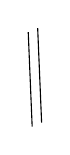
\begin{tikzpicture}\draw (0,0)--(0.05,-1.2);\draw (0.12,0.05)--(0.17,-1.15);\end{tikzpicture}}}
(de façon générale il est trivial que $V$ transforme $\unsure{\varinjlim}$ quelc. en $\varprojlim$).
Dans le cas de $F=V(M)$, ceci correspond donc aux hom
\[
M\xrightarrow{u}\operatorname{Sym}^*\left(\bigoplus N_\alpha\right)
=\bigotimes_\alpha\operatorname{Sym}^*(N_\alpha)
\]
Ici il y a lieu de décomposer $M$ suivant les multidegr. $i=(i_\alpha)_{\alpha\in I}\in\mathbb{N}^I$,
\diagram{
\begin{tikzcd}
u(\unsure{x|m})=\displaystyle\sum_{(i_\alpha)}\underbrace{u_{(i_\alpha)}(\unsure{x|m})} \\
\displaystyle\bigotimes_\alpha\operatorname{Sym}^{i_\alpha}(N_\alpha)\arrow[u,phantom,"\in" description,sloped]
\end{tikzcd}
}
\margin{145}
\scanpage{147}
on voit que si $\lambda=(\lambda_\alpha)\in\unsure{O_k}(A)^I$, $(x_\alpha^*)\in\left(\prod_{\alpha\in I}V(N_\alpha)\right)(A)$
\[
u^*((\lambda_\alpha x_\alpha^*)_{\alpha\in I})=(u^\lambda)^*(x_\alpha^*)
\]
i.e.
\[
u^*\prod_\alpha\lambda_{\alpha\,V(N_\alpha)}=(u^\lambda)^*\ ,
\]
où \deleted{$u^\lambda$ est}
\[
u^\lambda=\sum_{(i_\alpha)}\left(\prod_\alpha\lambda_\alpha^{i_\alpha}\right)u_{(i_\alpha)}
\]
Donc, si on se donne $\underline n=(n_\alpha)_{\alpha\in I}\in\mathbb{N}^I$, $u^*$ est multihomogène de \inserted{multi}degré $\underline n$ ssi on a
\[
u:M\longrightarrow\bigotimes_\alpha\operatorname{Sym}^{n_\alpha}(N_\alpha)
\]
En particulier, si tous les $n_\alpha$ sont égaux à 1, cela montre que $u^*$ est hom. de degré 1 en tous les arguments ssi
\[
u:M\longrightarrow\bigotimes_\alpha N_\alpha
\]
(en identifiant $N_\alpha$ à $\operatorname{Sym}^1N_\alpha$). Mais alors on constate tout de suite que $u^*$ est \inserted{$=$} multilinéaire (\unsure{pouvant} aussi se déduire formellement du cas d'1 variable (``en fixant les autres'')). Donc les accouplements bil.
\[
\prod V(N_i)\longrightarrow\deleted{\unsure{V(N}}M
\]
correspondent aux hom
\[
M\longrightarrow\bigotimes_\alpha N_\alpha
\]
en particulier les accouplements bil.
\[
V(N)\times V(N')\mathbin{\text{---}}V(M)
\]
correspondent aux hom
\[
M\mathbin{\text{---}}N\otimes N'.
\]
\margin{146}
\scanpage{148}
Faisant $M=N=N'$, on trouve qu'une loi de composition bilinéaire sur $V(M)$ correspond à un hom
\[
\Delta:M\mathbin{\text{---}}M\otimes M
\]
(appelé aussi ``application diagonale''). \deleted{On dit que}\inserted{on dit que $M$ \unsure{devt|devient} une coalgèbre.}
$\Delta$ est \unsure{coassociative|associative}, \inserted{resp.} commutative, \inserted{resp.} unitaire si la loi de composition sur $V(M)$ l'est.
\deleted{\unsure{l'unité}}\inserted{Cela} \unsure{s'explicite} par les diagrammes bien connus. Pour l'unitarité, on note que $e\in V(M)(k)$ s'identifie à une \uline{coaugmentation} ou counité
\[
M\xrightarrow{\unsure{\eta}}k
\]
(satisfaisant des conditions qu'on n'écrit pas, qui la définissent de façon unique).

Par contre, une \deleted{\unsure{la}} coaugmentation (multiplicative)
$V(M)\mathbin{\text{---}}O_k\inserted{=V(k)}$ correspond à un hom $k\mathbin{\text{---}}M$, ou encore un $\mathrm{él}^t$ de $M$ (appelé unité)
la condition ici est
\[
\Delta e=e\otimes e.
\]
Notons que par suite de la formule
\[
V\left(\lim_i M_i\right)=\deleted{\unsure{\prod_i}}\varprojlim_i V(M)
\]
(pour cat. d'indices quelc.), une lim. quelc. de coalgèbres est une coalgèbre, et les \deleted{structures}\inserted{axiomes} d'ass, d'unité, de comm.
\margin{147}
\scanpage{149}
passent à la limite.

Soit \deleted{$\unsure{Z}$} $\unsure{D|Z}$ un ens. Une graduation de type $D$ de $M$ est une décomposition en somme directe
\[
M\simeq\bigoplus_{d\in\unsure{D|Z}}M_d\qquad(M_d\text{ sous-module de }M)
\]
\deleted{\unsure{On interprète}}\inserted{\unsure{s'écrit}} aussi comme décomposition de $V(M)$ en produit
\[
V(M)\simeq\prod_{d\in\unsure{D|Z}}V(M_d)
\]
(modules quotients). Il est souvent commode aussi de regarder \deleted{la cat.}\inserted{(\unsure{cat. oppos. de cat.})} des \inserted{$M_*$} gradués par $D$ comme des familles $(M_d)_{d\in D}$ de $k$-modules, donc $V(M)_{\inserted{*}}$ comme la \uline{famille} des $V(M_d)$. $(d\in Z)$

Si $\unsure{D|Z}$ est muni d'une structure de groupe abélien, alors la structure dite sur $M$ revient à faire opérer le groupe diagonalisable de $\widehat C_k$
\diagram{
\begin{tikzcd}[column sep=large]
D(Z)=G: \arrow[d,phantom,"\wr" description] & A\arrow[r,phantom,"\unsure{-|\longmapsto}" description] & \operatorname{Hom}_{\mathrm{Ab}}(\unsure{D|Z},A^*)\arrow[d,phantom,"\wr" description]\\
\operatorname{Spec}k(Z) & & \operatorname{Hom}_{k\text{-Alg}}(\underbrace{k(Z)}_{\text{alg du groupe}},A)
\end{tikzcd}
}
\inserted{lin. sur}\deleted{sur} $M$ [\unsure{par quoi on entend} : sur $W(M):A\mathbin{\text{---}}M\otimes A$, ou au choix par
\margin{148}
\scanpage{150}
\unsure{contragrédience}, sur $V(M)$].

Une structure de coalg $\Delta$ sur $M$ est dite \uline{compatible} avec la graduation, si
\[
\Delta:M\mathbin{\text{---}}M\otimes M
\]
est compatible avec la ``graduation totale''
\[
\left(\Delta(M_n)\subset\sum_{i+j=n}M_i\otimes M_j\right)
\]
ou, ce qui revient au $=$, si la loi de composition sur $V(M)$ est compatible avec les graduations, i.e. provient d'hom
\diagram{
\[
\begin{array}{ccccc}
V(M_i)&\times&V(M_j)&\longrightarrow&V(M_{i+j})\\
\text{\textquotedbl}&&\text{\textquotedbl}&&\text{\textquotedbl}\\
V(M)^i&\times&V(M)^j&&V(M)^{i+j}
\end{array}
\]
}
Il revient aussi de $=$ de dire que la multiplication dans $V(M)$ (ou la comultiplication de $M$) commute à l'action de $G$.
\margin{La donnée d'une telle $\Delta$ revient à la donnée des
\[
\Delta_n:M_n\mathbin{\text{---}}\sum_{i+j=n}M_i\otimes M_j
\]
i.e. de \deleted{$\unsure{\sum}$}
\diagram{\begin{tikzcd}
\displaystyle\prod_{i+j=n}\underbrace{V(M_i)\times V(M_j)}_{V(M)^i\times V(M)^j}\arrow[r] & V(M_{i+j})\arrow[d,phantom,"\Vert" description]\\
& V(M)^n
\end{tikzcd}}
}
\margin{\uline{NB} dans ce pt de vue ``familles des modules indexés par $\unsure{M_i}$'', au lieu des $\Delta_n$ il suffit de se donner des
\[
\Delta^{ij}:M_{i+j}\mathbin{\text{---}}M_i\otimes M_j,
\]
ou des accouplements
\[
V(M)^i\times V(M)^j\mathbin{\text{---}}V(M)^{i+j},
\]
\unsure{sans} condition loc. finitude. \unsure{on a des algèbres}\illegible{2}
}
Bien sûr, les (morph. de coalgèbres graduées) correspondent aux hom des $O_k$-Alg. correspondantes (éventuellement graduées).

Condition d'anticommutativité, lorsqu'on dispose d'un hom
\[
\deleted{\unsure{\varphi}}\quad Z\mathbin{\text{---}}\mathbb{Z}/2\mathbb{Z}
\]
(i.e. $\mu_2\mathbin{\text{---}}G$) qui permet de \deleted{\unsure{d'introduire à $M$}}\inserted{d'associer à la graduation donnée} une graduation de \deleted{de} groupe $\mathbb{Z}/2\mathbb{Z}$, idem pour $V(M)$,
\margin{149}
\scanpage{151}
On dit alors que $\Delta$ (ou la coalgèbre \inserted{$M$}) est anticommutative si \deleted{\unsure{tt}} la multiplication sur \deleted{$V(M)$} l'algèbre graduée
\[
\deleted{V(M)=V(M)^{\mathrm{pair}}}\qquad
V(M)=V(M)^{\mathrm{pair}}\times V(M)^{\mathrm{impair}}
\]
l'est, i.e. si on a (pour $x,y\in V(M)(A)$ hom mod 2)
\[
xy=(-1)^{\deg x\deg y}yx
\]
(i.e. $xy=yx$ si $x$ \unsure{ou|et} $y$ \deleted{ont $=$ degré mod 2}\inserted{sont de degré pair}, \deleted{$xy=yx$} $xy=-yx$ i.e. $xy+yx=0$ si l'un et l'autre de degré impair). On laisse au lecteur le soin de diagrammatiser cette condition.

On dit que $\Delta$ (ou la coalgèbre $M$) est alternée si la multiplication de $V(M)$ l'est, i.e. si on a pour \deleted{\unsure{alg $V$}} $x,y\in V(M)(A)$ homogènes\deleted{\unsure{et}} mod 2, on a
\[
\begin{cases}
xy=yx&\text{si }x\text{ ou }y\text{ de degré pair}\\
\textcircled{$x^2=0$}&\text{si }x\text{ de degré impair}
\end{cases}
\]
\margin{signifie que le composé
\[
\deleted{\unsure{M^{\mathrm{imp}}\longrightarrow1}}
\]
\diagram{\begin{tikzcd}
\unsure{M^0}\arrow[r,"\unsure{\Delta^{00}|\Delta^{11}}"] & M^1\otimes M^1\arrow[r] & \operatorname{Sym}^2M^1
\end{tikzcd}}
est nul (degrés mod 2)
}
(alors, si $x$ et $y$ de degré impair, utilisant $x^2=y^2=(x+y)^2=0$, on trouve $xy+yx=0$, donc l'Algèbre est anticommu., donc \inserted{pour} la coalgèbre aussi
\[
\text{alternée}\ \Longrightarrow\ \text{anticommutative}.
\]
Bien sûr, anticommutativité et \inserted{le caractère} alterné \deleted{\unsure{procèdent}} des \deleted{\unsure{tt fait}} coalgèbres se conservent par \uline{lim} quelc.

On définit les $k$-\inserted{co}dérivations d'une coalgèbre, et les $k$-antidérivations (tjrs
\margin{150}
\scanpage{152}
supposées de degré impair, i.e. échangeant parité des degrés) pour des coalgèbres, comme correspondant aux dérivations resp. antidérivations de la $O_k$-Algèbre $V(M)$ (\unsure{évt|cat.} graduée mod 2). On a donc que le crochet de deux dérivations est une dérivation, l'anti-crochet de deux antidérivations est une antidérivation. On notera que si $\unsure{d}$ (revenant à un groupe de degrés quelc.) un endom. $d$ de $M$ est de degré $\gamma$, alors l'endom correspondant de $V(M)$ est de degré $-\gamma$ --- sauf si on change les degrés \inserted{de signe} pour l'objet
\diagram{\[
\begin{array}{ll}
V(M_i)&=V(M)^i=V(M)_{-i}\\
\text{\textquotedbl}&\\
V(M^{-i})&
\end{array}
\]}
Mais pour les histoires de dérivations \inserted{et antidérivations}\deleted{il est} seul un degré mod 2 importe, donc il n'y a pas alors à distinguer entre degré $i$ et $-i$ d'un endom. linéaire.

On traite de façon analogue les ``copuissances divisées'', \deleted{\unsure{un ``coidéal'' d'une coalgèbre}}\inserted{modules sur, sous-coalgèbre d'une} coalgèbre --- Pour le faire avec la généralité qui convient (pas seulement dans le cas commu., \deleted{\unsure{\&}} mais aussi le cas anticommu.) il faut d'abord disposer des \unsure{notions} dans le cas pas ``co'', mais ordinaire.
\margin{151}
\scanpage{153}
\figure{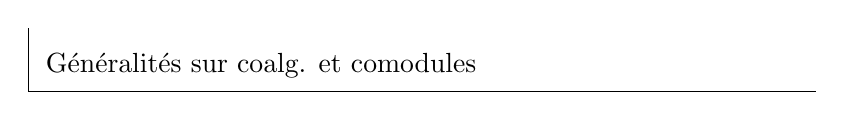
\begin{tikzpicture}\node[anchor=south west] at (.1,.05) {Généralités sur coalg. et comodules};\draw (0,.8)--(0,0)--(10,0);\end{tikzpicture}}

Soit $s$ une $k$-coalg (\deleted{\unsure{commu}}, ass \unsure{unit})
$C$ un comodule \inserted{à g.} sur $s$
donc $V_k(C)$ est un Module \inserted{\unsure{à d.}} sur $V_k(s)$ ; \deleted{\unsure{qui}} donc \inserted{l'Alg.} $V_k(s)$ opère \inserted{\unsure{à d.}} sur $V_k(C)$ ; donc l'algèbre $V_k(s)(k)=s^k$ opère \inserted{\unsure{à d.}} sur $V_k(C)$, donc à droite sur $C$. Donc $C$ est un module \inserted{à droite} ordinaire sur $s^k$, et sa structure de $k$-module s'en déduit (par $k\longrightarrow s^k$).

Quand peut-on récupérer la structure de comodule \inserted{(à g.)} sur $s$, connaissant la structure de module (à dr.) sur $s^k$ ? [NB. il est clair que si on connaît la structure de module à dr. de $C\otimes_k k'$ sur $s^{k'}$ $\forall k'$, alors on connaît la structure de comodule de $C$ sur $s$ ; de façon plus précise, une telle structure de comodule à g. \deleted{\unsure{revient}} \unsure{est la} donnée d'une structure de module, droite de
\[
W(C)=(k'\longmapsto C\otimes_k k')
\]
sous
\[
V(s)=(k'\longmapsto s^{k'}=\operatorname{Hom}_{k\text{-mod}}(s,k').
\]
] Soit $u\in s^k$, $u:s\mathbin{\text{---}}k$, alors l'op. $u_C$ de $u$ sur $C$ est le composé
\diagram{\begin{tikzcd}
C\arrow[r,"\Delta_C"]\arrow[rr,bend right=25,"u_C"'] & C\otimes s\arrow[r,"\mathrm{id}_C\otimes u"] & C\otimes k\simeq C
\end{tikzcd}}
donc la connaissance des $u_C$ équivaut à la connaissance du composé
\diagram{\begin{tikzcd}
C\arrow[r,"\Delta_C"] & C\otimes s\arrow[r,"\mathrm{id}_C\otimes u"] & \displaystyle\prod_{u\in s^k}C\otimes k
\end{tikzcd}}
et tt est bien si $C\otimes s\mathbin{\text{---}}\prod_{u\in s^k}C\otimes k$ est injectif.
\margin{152}
\scanpage{154}
\begin{center}- 113 -\end{center}
\margin{IX}

9.4.7.3. Cet énoncé garde un sens et reste valable lorsqu'on suppose seulement que $S$ est un schéma noethérien régulier connexe de dimension 1 : au lieu d'un seul accouplement (9.4.7.2), il faut alors considérer un accouplement $Q_s\otimes Q_s^*\longrightarrow\Lambda_s$ pour chaque point fermé $s$ de $S$. C'est sous cette forme plus générale qu'il nous sera le plus commode de prouver 9.4.7.

a) Pour toute extension panachée $X$, l'application
\[
\operatorname{End}(X)\longrightarrow\operatorname{End}(X_\eta)
\]
est bijective. Comme les deux membres sont respectivement les sections de $\uline{\operatorname{Hom}}(P,Q)=D(Q\otimes Q^*)$ sur $S$ et sur $\eta$, l'assertion provient du fait que $S$ est normal et que $D(Q\otimes Q^*)$ est fini sur $S$. De ceci résulte aussitôt que si $X$ et $Y$ sont deux extensions panachées, et si on sait déjà qu'elles sont isomorphes, alors
\[
\uline{\operatorname{Hom}}(X,Y)\longrightarrow\uline{\operatorname{Hom}}(X_\eta,Y_\eta)
\]
est bijectif.

b) Si $X$ et $Y$ sont deux extensions panachées, tout isomorphisme $X_\eta\xrightarrow{\sim}Y_\eta$ provient d'un isomorphisme $X\longrightarrow Y$. Grâce à a) la question est locale pour la topologie étale, ce qui nous permet de nous ramener au cas où $S$ est strictement local. Mais dans ce cas 9.4.3 nous montre que l'application
\margin{\unsure{ON}}
\[
\operatorname{Ext}^1_\Lambda(P,Q)\longrightarrow\operatorname{Ext}^1_\Lambda(P_\eta,Q_\eta)
\]
s'identifie à l'application
\[
V^*\otimes\check H_{\unsure{o|0}}\longrightarrow K^*\otimes\check H_{\unsure{o|0}}
\]
\margin{431}
\margin{431}
\margin{153}
\scanpage{155}
Si $C$ est plat sur $k$, et $s\hookrightarrow k^I$ pour $I$ convenable
i.e. $s\mathbin{\text{---}}k^{s^k}$ $(x\longmapsto(u(x))_{u\in s^k})$ est injectif,
alors $C\otimes s\mathbin{\text{---}}C\otimes_{\unsure{s|k}}k^I$ est injectif, mais
\diagram{\[
\begin{array}{rclll}
C\otimes_k k^{(I)}&\longrightarrow&(C\otimes_k k)^I=&C^I&\text{est-il injectif ?}\\
&&&\text{\textquotedbl}&\\
&&&\operatorname{Hom}(k^{(I)},C).&
\end{array}
\]}
\uline{Oui}, par passage à la limite inductive sur $I$, on se ramène au cas $I$ fini\unsure{---}.
\figure{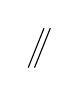
\begin{tikzpicture}\draw (0,0)--(.2,.5);\draw (.08,0)--(.28,.5);\end{tikzpicture}}
\unsure{Même conclusion} sans hyp. de platitude sur $C$ en supposant que $s$ est \uline{libre} sur $k$\ldots
\figure{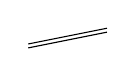
\begin{tikzpicture}\draw (0,0)--(1,.2);\draw (0,-.05)--(1,.15);\end{tikzpicture}}
\[
 s=k[U].\qquad s^k=k\{\{T\}\}
\]
structure de $k$-Alg. ordinaire
\[
 \begin{aligned}
 C&=k[U][Y_0,\ldots,Y_n]\\
  &=k[U,Y_0,\ldots,Y_n]
 \end{aligned}
 \qquad C^k=k\{\{T\}\}\{\{X_0,\ldots,X_n\}\}
\]
structure de $k$-Alg. ordinaire qui est une $s^k$-Alg.

$C^k$ opère sur $C$ par les
\[
 T^{(i)}X_0^{(i_0)}\cdots X_n^{(i_n)}
\]
qui \unsure{op. par} les op. diff.
\[
 D_U^{(i)}D_{Y_0}^{(i_0)}\cdots D_{Y_n}^{(i_n)}
\]
\deleted{\unsure{NB}} Donc $s^k$ opère par les $D_U^{(i)}$.

\uline{Remarque} Toutes ces opérations sont \inserted{loc.}\uline{nilpotentes}, de façon précise si $P\in C$ fixé, $P$ de degré $n$,
alors $D_fP=0$ si $f\in C^k$ est d'\uline{ordre} $>n$,
a fortiori si $f\in s^k$ d'ordre $>n$.
\figure{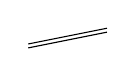
\begin{tikzpicture}\draw (0,0)--(1,.2);\draw (0,-.05)--(1,.15);\end{tikzpicture}}
Supposons $s$ $k$-coalgèbre (coassociatif, unitaire)
libre comme $k$-module, quelles sont les structures de $s^k$-algèbre sur \inserted{le $k$-module} $C$ qui
proviennent d'une structure de $k$-comodule ?
\diagram{\begin{tikzcd}[column sep=large]
 C\arrow[r] & C\otimes_k s\arrow[r,phantom,"\subset" description,"{\text{inj. car }s\text{ libre -- cf ci-dessus}}" above]\arrow[dr] & \operatorname{Hom}_k(s^k,C)\\
 &&\deleted{C\otimes_k\underbrace{\operatorname{Hom}_k(s^k,k)}_{(s^k)^k}}\arrow[r] & \deleted{\operatorname{Hom}_k(s^k,C\otimes k)}
\end{tikzcd}}
\margin{154}
\scanpage{156}
\margin{155}
\begin{center}- 112 -\end{center}\hfill IX

Revenant à la définition de (9.4.2) lorsque $S$ est strictement local, on note que la relation $\operatorname{Ext}^2(Q,P)=0$ implique la possibilité de définir un élément canonique (9.3.13), où on prend pour $Y'$ l'extension panachée $X_\eta$ donnée de $E_\eta$ par $F_\eta$. La formule (9.4.5) permet d'identifier cet élément $c(X_\eta)$ à un élément de $\check Q_{\unsure{o|0}}\otimes\check Q_{\unsure{o|0}}^*$, ce qui précise la définition de (9.4.2). On trouve de plus, en vertu des considérations générales de 9.3, que l'élément en question s'interprète comme l'obstruction au prolongement de $X_\eta$ en une extension panachée $X$ de $E$ par $F$.

9.4.6. La définition de (9.4.1) dans le cas $S$ hensélien se ramène maintenant immédiatement au cas strictement local, par descente galoisienne à partir du hensélisé strict de $S$.

\uline{Proposition} 9.4.7. \uline{Les données} $P,Q,R,E,F$ \uline{sont comme ci-dessus}, \uline{sauf qu'il est inutile de supposer le trait} $S$ \uline{hensélien}. \uline{On considère le foncteur}
\figure{\begin{tikzpicture}\draw (0,.3)--(.12,0);\end{tikzpicture}}
\[
 (9.4.7.1)\qquad X\longmapsto X_\eta
\]
\uline{de la catégorie des extensions panachées de} $E$ \uline{par} $F$ \uline{dans la catégorie des extensions panachées de} $E_\eta$ \uline{par} $F_\eta$. \uline{Pour toute extension panachée} $X_\eta$ \uline{de} $E_\eta$ \uline{par} $F_\eta$, \uline{on considère l'accouplement}
\[
 (9.4.7.2)\qquad c_{\unsure{o|0}}(X_\eta):Q_{\unsure{o|0}}\otimes Q_{\unsure{o|0}}^*\longrightarrow\Lambda_{\unsure{s|S}}
\]
\uline{induit par l'accouplement du type} (9.4.1) \uline{défini sur le} hensélisé $S^h$ \uline{de} $S$.

\uline{Ceci posé}, \uline{le foncteur} (9.4.7.1) \uline{est} pleinement fidèle, \uline{et pour une extension panachée} $X_\eta$ \uline{de} $E_\eta$ \uline{par} $F_\eta$, $X_\eta$ \uline{appartient à l'image essentielle de ce foncteur si et seulement si l'accouplement} (9.4.7.2) \uline{est nul}.
\margin{\diagram{\begin{tikzcd}\unsure{\otimes^i k}\arrow[r]&\unsure{\wedge}\end{tikzcd}}}
\margin{430}
\margin{430}
\scanpage{157}
On voit que c'est OK ssi $\forall x\in C$, l'application
\[
 \unsure{i_x|\iota_x}:u\longmapsto u_Cx,\qquad s^k\mathbin{\text{---}}C
\]
est dans $C\otimes_k s$, \deleted{\unsure{ssi}} i.e. (\unsure{en termes} d'une base $(e_\alpha)_{\alpha\in A}$ de $s$) se met sous la forme
\[
 u_Cx=\left(\sum_{\substack{\text{somme finie}\\x_\alpha\in C}}x_\alpha\otimes e_\alpha\right)(u)
 =\sum u(e_\alpha)x_\alpha
\]
ou encore, en posant
\[
 u(e_\alpha)=u_\alpha\qquad\text{donc }u\longmapsto(u_\alpha)_{\alpha\in A}\qquad s^k\simeq k^A
\]
\[
 u.x=\sum u_\alpha x_\alpha.
\]
\figure{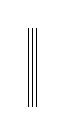
\begin{tikzpicture}\draw (0,0)--(0,1);\draw (.05,0)--(.05,1);\draw (.10,0)--(.10,1);\end{tikzpicture}}
Cela signifie aussi que $u\longmapsto u.x$ est continue pour la top. discrète sur $C$ et la top. de la convergence simple sur $s^k$.

Ou encore que
\[
 s^k\mathbin{\text{---}}\operatorname{Hom}_k(C,C)
\]
est continue, \unsure{qd} on met des deux côtés la top. de la conv. simple-discrète\ldots
\figure{\begin{tikzpicture}\draw (0,0)--(1,.2);\end{tikzpicture}}
Supposons maintenant que $s$\inserted{$=\sum s_n$} soit gradué
(pour $\Delta$) donc $s^k$ gradué,
\diagram{\begin{tikzcd}
s^k=\displaystyle\prod_{n\in D}s_n^k\arrow[r,phantom,"=" description]\arrow[r,bend right=35,"\mathrm{dfn}"'] & \displaystyle\prod_{n\in D}(s^k)_n.
\end{tikzcd}}
Soit $C$\inserted{$=\sum_{n\in D}C_n$} comodule gradué --- donc
\inserted{$C^k=\prod(C_n)^k=\prod(C^k)_n$}
\deleted{\unsure{co}}module gradué sur
\[
 s^k=\prod(s^k)_n=\prod(\unsure{C_n^k|s_n^k}).
\]
Alors \deleted{si $u\in s^k$ \unsure{$0$}} si $u\in(s^k)_n$,
\[
 (u_C)^k:\unsure{V(C_m^k)|C_m^k}\mathbin{\text{---}}\unsure{V(C_{m+n})|(C_{m+n})^k}
\]
donc
\[
 u_C:C_{m+n}\mathbin{\text{---}}C_m
\]
i.e. $u_C$ \uline{diminue} les degrés de $n$ ! (Pour qu'il les augmente il faut changer de signe les degrés de $C$ et plutôt exiger que
\[
 V(C)^m\overset{\mathrm{dfn}}=V(C_{-m})
\]
\unsure{---})
\margin{156}
\scanpage{158}
\begin{center}- 111 -\end{center}\hfill IX

Reste à décrire des isomorphismes d). En fait, sur une base quelconque $U$, on a un homomorphisme canonique
\[
 (9.4.3.1)\qquad \mathbb G_m(U)\otimes\check H_{\unsure{o|0}}\longrightarrow H^1(U,D(H_{\unsure{o|0}U}))\ ,
\]
qu'on décrit, lorsque $H_{\unsure{o|0}}$ est annulé par l'entier $m\geq0$, à l'aide de l'homomorphisme cobord $\mathbb G_m(U)\xrightarrow{\partial}H^1(U,\mu_m)$ associé à la suite exacte de Kummer, en prenant le composé
\diagram{\begin{tikzcd}[column sep=small]
 \mathbb G_m(U)\otimes\check H_{\unsure{o|0}}\arrow[r]& H^1(U,\mu_m)\otimes\check H^{\unsure{o|0}}\arrow[r]& H^1(U;\mu_m\otimes\check H_{\unsure{o|0}})\arrow[r]&H^1(U,D(H_{\unsure{o|0}S}))\ ,
\end{tikzcd}}
où la deuxième flèche se déduit de l'homomorphisme évident $\check H_{\unsure{o|0}}\longrightarrow\operatorname{Hom}(\mu_m,\mu_m\otimes\check H_{\unsure{o|0}})$, et la troisième est un cas particulier de b) (où on remplace $n$ par $m$). Nous laissons au lecteur le soin de vérifier que (9.4.3.1) ne dépend pas du choix de l'entier $m$ tel que $mH_{\unsure{o|0}}=0$.
D'autre part je dis que l'homomorphisme (9.4.3.1) est toujours injectif, et que son conoyau est nul si $\operatorname{Pic}(U)=0$. (En fait, le conoyau est toujours isomorphe à $\operatorname{Hom}(H_{\unsure{o|0}},\operatorname{Pic}(U))$, mais peu importe ici.) Pour voir ceci, on est ramené en effet au cas où $H_{\unsure{o|0}}$ est de la forme $\mathbb Z/n\mathbb Z$, et alors l'assertion résulte aussitôt de la suite exacte de cohomologie associée à la suite exacte de Kummer (*) ci-dessus. Ceci prouve la formule d). On en conclut aussitôt :

\uline{Corollaire} 9.4.4. \uline{Avec les notations de} 9.4.3 \uline{on a un isomorphisme canonique}
\[
 \text{e)}\qquad H^1(\eta,D(H)_\eta)/\operatorname{Im}H^1(S,D(H)\simeq\check H_{\unsure{o|0}}\ ,
\]
\uline{d'où} (\uline{en combinant avec} a) \uline{et} b)) \uline{un isomorphisme canonique}
\figure{\begin{tikzpicture}\draw (0,0)--(.15,.25)--(.35,0);\end{tikzpicture}}
\[
 (9.4.5)\qquad\operatorname{Ext}^1(Q_\eta,P_\eta)/\operatorname{Im}\operatorname{Ext}^1(Q,P)\simeq\check Q_{\unsure{o|0}}\otimes\check Q_{\unsure{o|0}}^*\ .
\]
\margin{\figure{\begin{tikzpicture}\draw (0,.1)--(.45,.1) (.35,.28)--(.38,0);\draw (.85,.18)--(.9,0);\draw (5.5,0)--(5.6,.17)--(5.7,0);\end{tikzpicture}}}
\margin{429}
\margin{429}
\margin{157}
\scanpage{159}
Donc la catégorie des $s$-comodules gradués équivaut à la catégorie des $s^k$-modules gradués $C$ \deleted{\unsure{plats}} qui sont ``\deleted{loc.} \uline{intégrables}''
i.e. tels que $\forall x\in C$, $u\longmapsto u.x$ de $s^k$ dans $C$ est continue pour la conv. simple sur $s^k$ ($=$ top \unsure{produit} sur $k^A$)
\margin{158}
\scanpage{160}
\margin{159}
\margin{$\unsure{u\in}(s^k)^n=(s_{-n})^k$
\diagram{\begin{tikzcd}
 u:\ V(C_{\deleted{\unsure{m}}})^m\arrow[r]\arrow[d,equal]&V(C)^{m+n}\arrow[d,equal]\\
 \unsure{V}(C_{-m})&V(C_{-m-n})
\end{tikzcd}}}
\figure{\begin{tikzpicture}\draw (0,0)--(.7,2);\end{tikzpicture}}
\begin{center}- 110 -\end{center}\hfill IX

Ceci est un cas particulier du

\uline{Lemme} 9.4.3. \uline{Sous les conditions précédentes}, \uline{avec} $S$ \uline{strictement local, on a des isomorphismes}
\[
 \text{a)}\quad\operatorname{Ext}^i_\Lambda(Q,P)\simeq H^i(S,\check Q\otimes P)\ ,\quad
 \operatorname{Ext}^i_\Lambda(Q_\eta,P_\eta)\simeq H^i(\eta,\check Q\otimes P)\ ,
\]
\uline{d'autre part on a un isomorphisme canonique}
\[
 \text{b)}\qquad\check Q\otimes P\simeq D(Q\otimes Q^*)\ ,
\]
\uline{enfin}, \uline{pour tout groupe constant fini} $H=H_{\unsure{o|0}S}$ \uline{sur} $S$, \uline{on a}
\[
 \text{c)}\qquad H^i(S,D(H)\unsure{=|\simeq}H^i(\eta,D(H)_\eta)=0\quad\text{\uline{pour} }i\geq2\ ,
\]
\uline{et des isomorphismes canoniques}
\[
 \begin{aligned}
 \text{d)}\quad H^1(S,D(H))&\simeq\mathbb G_m(S)\otimes\check H_{\unsure{o|0}}=V^*\otimes\check H_{\unsure{o|0}}\ ,\\
 H^1(\eta,D(H_\eta))&\simeq\mathbb G_m(\eta)\otimes H_{\unsure{o|0}}=K^*\otimes\check H_{\unsure{o|0}}\ ,
 \end{aligned}
\]
\uline{où le signe} $\vee$ \uline{désigne ici} $\operatorname{Hom}(-,Q/\mathbb Z)$.

Les formules a) et b) résultent trivialement du fait que $Q$ est un $\Lambda_S$-Module localement libre de type fini. Pour prouver c), on est évidemment ramené au cas où $H_{\unsure{o|0}}=\mathbb Z/m\mathbb Z$ i.e. $D(H)=\mu_m$, et alors la \unsure{auite|suite} exacte de cohomologie associée à la suite exacte de Kummer
\diagram{\begin{tikzcd}
 0\arrow[r]&\mu_m\arrow[r]&\mathbb G_m\arrow[r,"{m.\mathrm{id}}"]&\mathbb G_m\arrow[r]&0
\end{tikzcd}}
nous ramène à prouver les formules
\[
 H^i(S,\mathbb G_m)=H^i(\eta,\mathbb G_m)=0\quad\text{pour }i\geq1\ .
\]
Les $H^i$ sont égaux aux $H^i_{\mathrm{\acute et}}$ calculés pour le site étale [6, th. 11.7], ils sont donc nuls pour $S$ puisque $S$ est strictement local. Le fait qu'ils sont nuls aussi pour $\eta$ est un fait bien connu [6, th. 1.1].
\margin{$\unsure{\Lambda|A}$}
\margin{428}
\margin{428}
\scanpage{162}
\margin{\figure{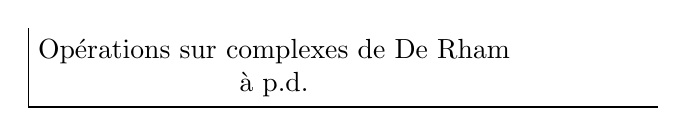
\begin{tikzpicture}\node[align=center,anchor=south west] at (0,0) {Opérations sur complexes de De Rham\\à p.d.};\draw (0,1)--(0,0)--(8,0);\end{tikzpicture}}}
\deleted{Proposition}
\uline{Théorème} Soient $(S,S^+,t)$ et $(S',S'^+,t')$ deux anneaux (comm.) à idéal à p.d. et élément marqué dedans
(\uline{\unsure{ps}} $S^+=(t)_{\mathrm{p.d.}}$, $S'^+=(t')_{\mathrm{pd}}$)
d'où
\[
 \begin{array}{ccc}\mathcal A(S,S^+,t)_*&\text{et}&
 \mathcal A'(S',S'^+,t')_*\\
 \Vert&&\Vert\\
 \mathcal A_S&&\mathcal A_{S'}\end{array},
\]
qu'on considère comme anneaux différentiels \unsure{$\tfrac12$|$k$}-simpliciaux
(faisant abstraction de leurs structures graduée, filtrée, à p.d., et de $S$ et $S'$ algèbres\ldots).
Alors les hom \inserted{$\varphi$} de tels anneaux \inserted{différentiels \unsure{$\tfrac12$|$k$}-simpliciaux} correspondent biunivoquement aux systèmes $(\varphi_0,A'_{\deleted{1}},(B'_i)_{i\geq1})$, où
\[
 \left\{\begin{aligned}
 &\varphi_0:S\mathbin{\text{---}}S'\quad\text{un hom d'anneaux}\\
 &A'_{\deleted{1}}\in S'\{X_0\}^{++}=\operatorname{Ker}(\alpha_{S'}:S'\{X_0\}\mathbin{\text{---}}S';\ \alpha(X_0^{(i)})=0\quad\forall i\geq1)\\
 &B'_i\in S'\{X_0\}
 \end{aligned}\right.
\]
sont donnés en fonction de $\varphi$ par
\[
 \left\{\begin{aligned}
 &\varphi_0=\text{composante de degré }0\text{ de }\varphi,\\
 &A'_{\deleted{1}}=\unsure{K_0|\pi_0}\varphi_1(X_0)\\
 &B'_i=\unsure{K_1|\pi_1}\varphi_1(X_0^{(i)})
 \end{aligned}\right.
\]
\diagram{\begin{tikzcd}
 \varphi_0:(\mathcal A_S)_0\arrow[r,dash]\arrow[d,equal]&(\mathcal A_{S'})_0\arrow[d,equal]\\
 S&S'
\end{tikzcd}}
\diagram{\begin{tikzcd}
 \varphi_1:S\{X_0\}\deleted{[dX_0]}\arrow[r]\arrow[d,equal]&S'\{X_0\}[dX_0]\arrow[d,equal]\\
 (\mathcal A_S)_1&(\mathcal A_{S'})_1
\end{tikzcd}}
$\unsure{K_0|\pi_0},\unsure{K_1|\pi_1}$ les projections sur les composantes de degré $0$ resp. $1$

\inserted{$(\varphi_0,A'_1,B'_i\ (i\geq1))$}
satisfaisant aux conditions
\[
 \left\{\begin{aligned}
 1)\quad&\deleted{\unsure{f_i}}\ \varphi_0(t^{(i)})=\varphi_0(t)^{(i)}
 &&\text{i.e. }\varphi_0\text{ commute aux p.d. sur }(t)_{\mathrm{pd}}\ (!)\\
 2)\quad&\beta_{S'}(A'_{\deleted{1}})=\varphi_0(t)
 &&\text{i.e. si }A'_{\deleted{1}}=\sum_{j\geq1}a'_{\deleted{1}j}X_0^{(j)},\text{ on a}\\
 &\sum_{j\geq1}a'_j t'^{(j)}=\varphi_0(t)\\
 3)\quad&(2^{\unsure{i|*}}B'_i)J'=0\ \deleted{\unsure{(A',B'_j)}}
 &&\forall i\geq1,
 \end{aligned}\right.
\]
où $J'$ est l'idéal de $S'$ engendré par les coeff. $a'_j$ de $A'$ et les coeff. $b'_{jh}$ des
\[
 B'_j=\sum_{h\geq0}b'_{jh}X_0^{(h)}.
\]
\margin{\uline{NB} dans la suite, supprimer l'indice $1$ à $A'_1$}
[\uline{NB} Si $\varphi_0(t)$ est \deleted{un élément} \inserted{\unsure{élémt} régulier} de $S'$ alors en vertu de \unsure{(2)} $J$ contient un élément régulier et les relations \unsure{(3)}
\margin{TSVP $\longrightarrow$}
\margin{161}
\scanpage{163}
\margin{365}
(3) signifient que
\figure{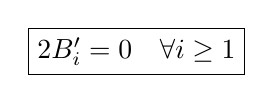
\begin{tikzpicture}\node[draw,rectangle] {$2B'_i=0\quad\forall i\geq1$};\end{tikzpicture}}
]. Il en est de même si $\varphi_*$ est un isom
($\Leftrightarrow$ \unsure{$\varphi_0$ et $\varphi_1$} un isom) car alors on voit que le coefficient dominant $a'_1$ de $\unsure{A_1|A'}(X_0)=a'_1X_0+\unsure{\mathbin{\text{---}}}$ est inversible dans $S'$.
Aussi dans les conditions du cor. 5, si $(\varphi_0(T))_{\mathrm{pd}}=(T')_{\mathrm{pd}}$ i.e.
\[
 \varphi_0(T)=\sum_{i\geq1}\lambda_i T'^{(i)}
\]
avec $\uline{\lambda_1}$ \uline{inversible}, alors \unsure{en} vertu de (2) on \unsure{trouve}
\[
 a'_1\equiv1\bmod\unsure{S_{k'}^+|S'^+}
\]
donc $a'_1$ est élément régulier \unsure{dans ce cas}.
Ainsi (3) s'écrit encore
\figure{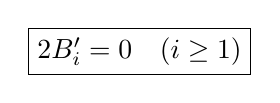
\begin{tikzpicture}\node[draw,rectangle] {$2B'_i=0\quad(i\geq1)$};\end{tikzpicture}}
\margin{$\unsure{\longrightarrow92|292}$}

\begin{center}- 47 -\end{center}\hfill IX

cette filtration induit une filtration analogue de $U(\ell)=U_\ell\otimes_{\mathbb Z_\ell}\mathbb F_\ell$, dont les facteurs successifs sont déduits des facteurs $V_i$ $(i=1,2,3)$
\[
 U^{\mathrm{et}},\quad U^{\mathrm{ef}}/U^{\mathrm{et}},\quad U/U^{\mathrm{ef}}
\]
intervenant dans la filtration (4.1.1) par tensorisation par $\mathbb F_\ell$. Bien entendu, cette filtration est stable sous $\Gamma$, et donne par additivité une décomposition de $\operatorname{long}\operatorname{Hom}_{\mathbb Z_\ell(\Gamma)}(L,U(\ell))$ en somme de trois termes, longueurs des groupes
\[
 (*)\quad\operatorname{Hom}_{\mathbb Z_\ell(\Gamma)}(L,V_i\otimes_{\mathbb Z_\ell}\mathbb F_\ell)
 \simeq(\operatorname{Hom}_{\mathbb Z_\ell(\Gamma)}(L,V_i))\otimes_{\mathbb Z_\ell}\mathbb F_\ell\ ,
\]
l'isomorphisme écrit dans (*) résultant encore de l'hypothèse de projectivité faite sur $L$ ; on suppose seulement $K'$ choisi assez grand pour que $\Gamma$ opère sur les $V_i$. Or $\operatorname{Hom}_{\mathbb Z_\ell(\Gamma)}(L,V_i)$ est évidemment un $\mathbb Z_\ell$-module sans torsion, donc son \uline{rang} est égal au deuxième membre de (*). Si $\varphi_i$ est le caractère de la représentation de $\Gamma$ dans $V_i$, et $\psi$ le caractère de la représentation de $\Gamma$ dans $\check L$, on trouve donc
\[
 \begin{aligned}
 (4.6.1)\quad\operatorname{long}\operatorname{Hom}_{\mathbb Z_\ell(\Gamma)}(L,U(\ell))
 &=\sum_{1\leq i\leq3}N^{-1}\sum_{g\in\Gamma}\psi(g)\varphi_i(g)\\
 &=N^{-1}\sum_{g\in\Gamma}\psi(g)\varphi(g),\quad\text{avec }N=\operatorname{card}\Gamma,
 \end{aligned}
\]
où $\varphi(g)=\sum\varphi_i(g)$ est aussi la fonction sur $\Gamma$ déduite par passage au quotient de la fonction sur le groupe d'inertie $I$ caractère de la représentation de monodromie de $I$ sur $U$. Or en vertu de 4.3 a) ce caractère est une fonction à \uline{valeurs entières rationnelles indépendante} de $\ell$.
Prenant $L=\mathrm{Sw}$, il en est de même du caractère $\psi(g)$ de $L$, qui est égal à $a-N\delta+1$, où $\delta$ est la ``\uline{fonction de Dirac}'' de $\Gamma$, et $a$ le ``\uline{conducteur}
\margin{162}
\scanpage{164}
On reconstitue $\varphi_*$\deleted{\unsure{$\mathcal A$}} à partir de
\diagram{\[\begin{array}{ccc}\varphi_0,&A'_1,&B'_i\ (i\geq1)\\&\Vert&\\&\sum_{j\geq1}a'_jX_0^{(j)}&\end{array}\]}
par
\[
 \left\{\begin{aligned}
 &\varphi_1(\lambda)=\varphi_0(\lambda)&&\text{si }\lambda\in S\\
 &\varphi_1(X_0^{(i)})=A_1'^{(i)}+B'_i\,dX_0\\
 &\varphi_1(dX_0)=dA'_1&&\left(=A_1'^{\mathrm{d\acute er}}dX_0,\text{ où }A_1'^{\mathrm{d\acute er}}=\sum_{j\geq1}a'_jX_0^{(j-1)}\right)
 \end{aligned}\right.
\]
et $\varphi_n$ (pour $n\geq2$) en posant
\[
 U_0=X_0,\ U_1=X_0+X_1,\ldots,\ U_{n-1}=X_0+X_1+\cdots+X_{n-1}
\]
(de sorte que
\[
 (\mathcal A_S)_n=S\{U_0,U_1,\ldots,U_n\}[dU_0,\ldots,dU_n],
\]
par
\[
 \left\{\begin{aligned}
 &\varphi_n(\lambda)=\varphi_0(\lambda)&&\text{si }\lambda\in S\\
 &\varphi_n(U_r^{(i)})=A_1'^{(i)}\{U_r\}+B'_i\{U_r\}\,dU_r
 &&\left(\begin{array}{c}0\leq r\leq n-1\\i\geq1\end{array}\right)\\
 &\varphi_n(dU_r)=dA'_1\{U_r\}\deleted{dU_r}=A_1'^{\mathrm{d\acute er}}\{U_r\}dU_r
 &&(0\leq r\leq n-1)
 \end{aligned}\right.
\]
[NB la condition $2B'_iJ'=0$ n'intervient pas pour construire $\varphi_1$, mais que pour $n\geq2$, pour assurer que si $0\leq r\ne s\leq n-1$, $\varphi_n(U_r^{(i)})$ \deleted{et $\varphi_n(dU_s)$} \inserted{commute} aux $\varphi_n(U_s^{(i)})$ et à $\varphi_n(dU_s)$\ldots\ \deleted{\unsure{commutent}}]

\uline{Corollaire 1} Si $2$ est inversible dans $S'$\inserted{et si l'une des 3 conditions \deleted{du} NB de la \unsure{page} après le \unsure{th.} (cf ``TSVP'')}, alors $\varphi_*$ respecte la structure graduée; si de plus $S^+=(t)_{\mathrm{pd}}$, $\varphi_*$ respecte la structure à p.d.

\uline{Corollaire 2} \inserted{Supposons $S^+=(t)_{\mathrm{pd}}$.} Pour que $\varphi$ commute aux p.d. il f. et s. qu'on ait
\[
 B'_i=A'_{\unsure{i|1}}{}^{(i-1)}B'_1\qquad\forall i\geq1
\]
(donc les $\varphi_*$ en question sont donnés par les systèmes $\varphi_0,A'_1,B'_1$ satisfaisant 1), 2) et $2B'_1\unsure{J'|J}=0$ (qui tient lieu de 3).
Pour que $\varphi$ respecte la graduation, il f. et s. que $B'_i=0$ $\forall i\geq1$. (donc les $\varphi$
\margin{163}
\scanpage{165}
\begin{center}- 46 -\end{center}\hfill IX

projectif implique que $\alpha_s(F_K)$ se comporte additivement pour les suites exactes.

Nous allons appliquer cette définition au cas du faisceau ${}_\ell A_K$, où $A_K$ est notre schéma abélien sur $K$. On a donc, dans ce cas, un entier
\[
 (4.5.4)\quad\alpha_s(A_K;\ell)=\operatorname{long}\operatorname{Hom}_{\mathbb Z_\ell(\Gamma)}(\mathrm{Sw},U_\ell\otimes_{\mathbb Z_\ell}\mathbb F_\ell),\quad U_\ell=T_\ell(A(\overline K)),
\]
$\Gamma$ étant choisi comme il a été dit (choix dépendant à priori de $\ell$).
L'entier (4.5.4) s'appelle l'\uline{exposant conducteur immodéré} (ou ``\uline{sauvage}'') (*) du schéma abélien $A_K$ par rapport à l'anneau de valuation discrète $V\subset K$ ; par passage au hensélisé, il est défini bien sûr sans supposer $V$ hensélien, et il se ramène aussitôt au cas où $S$ est \uline{strictement} local. Nous nous proposons de montrer le

\uline{Corollaire} 4.6. \uline{L'exposant conducteur immodéré} (4.5.4) \uline{ne dépend pas du choix du nombre premier} $\ell\ne p$.
\figure{\begin{tikzpicture}\draw (0,.12)--(.10,0);\draw (.03,.12)--(.13,0);\end{tikzpicture}}

Nous pouvons supposer $S$ strictement local. Nous allons donner le calcul de (4.5.4), en remplaçant $\mathrm{Sw}$ par n'importe quel autre $\mathbb Z_\ell(\Gamma)$-module projectif $L$. Notons que la filtration (4.1.1) de $U_\ell$ se fait par des sous-$\mathbb Z_\ell$-modules qui sont manifestement des facteurs directs, donc

\figure{\begin{tikzpicture}\draw (0,0)--(3,0);\end{tikzpicture}}
(*) Il y a lieu de définir aussi l'\uline{exposant conducteur modéré} de $A_K$ par rapport à $V$ comme l'entier différence des longueurs sur $\mathbb Z/\ell\mathbb Z$ des fibres géométriques générique et spéciale de ${}_\ell A^{\unsure{o|0}}$, qui est indépendant de $\ell$ et égal à $2\lambda+\mu$ avec les notations de (1.1.11) ; \uline{l'exposant conducteur} (total) de $A_K$ est défini comme la somme des deux entiers précédents; c'est le terme local qui intervient dans la formule d'Euler-Poincaré pour ${}_\ell A^{\unsure{o|0}}$ de SGA 5 X 6.2, [20].
\margin{$\unsure{\Lambda|A}$\quad\unsure{214|211}}
\margin{364}
\margin{164}
\scanpage{166}
commutent aux p.d. --- et ils sont donnés par les couples $(\varphi_0,A'_1)$ satisfaisant 1) et 2) [on peut oublier 3)]. ; \deleted{cette condition tjrs vérifiée si $2$ est \unsure{inv.} dans $S'$} !

\uline{Corollaire 3} Pour que $\varphi_*$ respecte la filtration \inserted{(croiss. gross.)}, il f. et s. que
\[
 A'_1\in\operatorname{Fil}^{1}\quad\text{et}\quad B'_i\in\operatorname{Fil}^{i-1}\quad\forall i\geq1
\]
\[
 A'_1=\underbrace{a'_1}_{\lambda}X_0,\qquad
 B'_i=b'_{i0}+b'_{i1}X_0\mathbin{\text{---}}+b'_{i,i-1}X_0^{(i-1)}
 \qquad(a'_1,b'_{ij}\in S')
\]
[donc la condition 2) devient
\[
 (2')\quad a'_1t'=\varphi_0(t)
\]
et 3)
\[
 (3')\quad(2b'_{ij})J'=0\quad(i\geq1,\ 0\leq j\leq i-1)
\]
].

Pour que $\varphi_*$ respecte la \uline{graduation} \uline{et} les filtrations il f. et s. qu'on ait
\[
 A'_1=a'_1X_0,\qquad B'_i=0\quad i\geq0,
\]
alors, si de plus on suppose $S^+=(t)_{\mathrm{pd}}$, ces $\varphi$ correspondent exactt aux couples
\[
 (\varphi_0,\lambda):\deleted{\unsure{S\xrightarrow{\varphi_0}S'}}\inserted{(S,S^+,t)\mathbin{\text{---}}(S',S'^+,t')},
\]
par prolongement canonique :
\[
 \mathcal A_{S*}\mathbin{\text{---}}\mathcal A_{S'*}\ !
\]
\uline{Cor 4} $\varphi_*$ respecte \uuline{tjrs} la filtration \uline{décroissante}, associée aux degrés extérieurs.
\figure{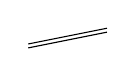
\begin{tikzpicture}\draw (0,0)--(1,.2);\draw (0,-.05)--(1,.15);\end{tikzpicture}}
Supposons maintenant
\[
 \begin{aligned}
 S&=k\{T\},&S^+&=(T)_{\mathrm{pd}},&t&=T\\
 S'&=k'\{T\},&S'^+&=(T)_{\mathrm{pd}},&t'&=T
 \end{aligned}
\]
\textcircled{1} La donnée de $\varphi_0$ correspond donc à la donnée de :
de \textcircled{a}
\[
 \varphi_{00}:k\mathbin{\text{---}}S'\deleted{\unsure{\{T\}}}=k'\{T\}
\]
(explicitable par un hom $k\xrightarrow{\delta_0}k'$ faisant de $k'$ un $k$-\unsure{module}) et des (\uline{op. diff.} $\delta_i$ $(i\geq1)$
\[
 \delta_i:k\mathbin{\text{---}}k'
\]
des tels que
\[
 \varphi_{00}(\lambda)=\sum_{i\geq0}\delta_i(\lambda)T^{(i)}
\]
On doit avoir
\[
 \begin{aligned}
 \delta_j(\unsure{1|u})&=0\quad j\geq1\\
 \delta_i(\lambda\lambda')&=\sum_{j+h=i}\unsure{C_{j,h}}\delta_j(\lambda)\delta_h(\lambda')\mathbin{\text{---}}
 \end{aligned}
\]
]
\margin{165}
\scanpage{167}
\begin{center}- 45 -\end{center}\hfill IX

\uline{correspondantes sont respectivement} $(q^n\epsilon_i)_{1\leq i\leq\mu}$ \uline{et} $(\epsilon_i)_{1\leq i\leq\mu}$, \uline{où les} $\epsilon_i$ $(1\leq i\leq\mu)$ \uline{sont des} racines de l'unité.

En fait, la formule (4.1.2) donne pour le dernier morceau les valeurs propres $q^n/(q^n\epsilon_i)=\epsilon_i^{-1}$, mais comme $\epsilon_i$ est une racine de l'unité, on a $\epsilon_i^{-1}=\overline{\epsilon_i}$ (conjugué complexe), et comme la famille des $\epsilon_i$ est stable par conjugaison complexe (comme famille des solutions d'une équation à coefficients entiers), la famille des $\epsilon_i^{-1}$ est aussi celle des $\epsilon_i$, ce qui prouve la dernière assertion de 4.4.

4.5. Nous allons donner une application de 4.3 a) à la théorie du conducteur local des schémas abéliens. Supposons $k$ algébriquement clos (*). Rappelons (SGA 5 X 6.2 ou [20])que pour tout schéma en $\ell$-groupes commutatifs étale $F_K$ sur $K$, $(\ell\ne p)$, on définit un entier
\[
 (4.5.1)\qquad\alpha_s(F_K)=\alpha_s(i_*(F_K))
\]
($i:\eta\longrightarrow S$ désignant l'inclusion), de la façon suivante : on choisit une extension galoisienne finie $K'$ de $K$, de groupe $\Gamma$, qui déploie $F_K$, de sorte que $F_K$ soit défini par un $\ell$-groupe fini $M$ sur lequel $\Gamma$ opère.
D'autre part, on associe à l'extension $K'$ de $K$ un certain $\mathbb Z_\ell[\Gamma]$-\uline{module projectif} (défini à isomorphisme près)
\[
 (4.5.2)\qquad\mathrm{Sw}=\mathrm{Sw}(K'/K,\mathbb Z_\ell)\ ,
\]
et on pose
\[
 (4.5.3)\qquad\alpha_s(F_K)=\operatorname{long}\operatorname{Hom}_{\mathbb Z_\ell(\Gamma)}(\mathrm{Sw},M)\ .
\]
On vérifie (loc. cit) que cette expression ne dépend pas du choix de l'extension $K'/K$. D'ailleurs, le fait que $\mathrm{Sw}$ soit un $\mathbb Z_\ell[\Gamma]$-module
\figure{\begin{tikzpicture}\draw (0,0)--(3,0);\end{tikzpicture}}
(*) Il suffirait en fait que $k$ soit \uline{parfait}, mais par passage au hensélisé strict de $S$, on se ramène aussitôt au cas envisagé.
\margin{\unsure{263|363}}
\margin{363}
\margin{166}
\scanpage{168}
\textcircled{b} $\varphi_0(T)\in S'^+$ \deleted{\unsure{quelc.}} mais sera fixé par condition 2)
\[
 \deleted{\varphi_0(T)=\sum_{i\geq1}\deleted{\unsure{\alpha_i}}\gamma'_iT^{(i)}\qquad(\gamma'_i\in k',\ i\geq1)}
\]
\deleted{\textcircled{2}} NB si on suppose qu'on se donne déjà $\psi=\varphi_{00}:k\longrightarrow k'$, et qu'on exige $\varphi_*$ $\psi$-semilinéaire i.e. $\varphi_0$ $\psi$-semi-linéaire, alors la donnée 1) se réduit à (b).

\textcircled{2}
\[
 A'_1\in S'_{\deleted{\unsure{*}}}\{X_0\}\simeq k'\{X_0,X_1\}
 =\sum_{\substack{\unsure{i,j\geq0}\\\deleted{\unsure{i\geq0}}\\j\geq0}}\alpha'_{ij}X_0^{(i)}X_1^{(j)}
\]
La condition $A'_1\in S'\{X_0\}^{++}$ signifie $\alpha'_{ij}=0$ si $i=0$
i.e.
\[
 A'_1=\sum_{\substack{i\geq1\\j\geq0}}\alpha_{ij}X_0^{(i)}X_1^{(j)}.
\]
On a
\[
 \beta_{S'}(A'_1)=\sum_{i\geq1}\alpha_{i,0}T^{(\unsure{j|i})},
\]
et on aura donc
\[
 \varphi_0(T)=\sum_{i\geq1}\alpha_{i,0}T^{(i)}
\]
\textcircled{3} $B'_i\in S'\{X_0\}\simeq k'\{X_0,X_1\}$ sont liés par la seule condition
\[
 (2B'_i)J=0.
\]
En résumé :

\uline{Cor. 5} Les hom. d'anneaux diff $\tfrac12$-simpliciaux
\[
 \mathcal A_{k*}=\mathcal A(k\{T\},k\{T\}^+,T)\mathbin{\text{---}}\mathcal A_{k'*}=\mathcal A(k'\{T\},k'\{T\}^+,T)
\]
sont définis par les systèmes \unsure{d'objts}
\[
 \left\{\begin{aligned}
 &\varphi_{00}:k\mathbin{\text{---}}k'\{T\}\quad\text{hom d'anneaux}\\
 &A'_{\deleted{1}}\in\deleted{\unsure{S'}}k'\{T\}\{X_0\}^{\deleted{++}}\simeq k'\{X_0,X_1\}\\
 &B'_i\in k'\{T\}\{X_0\}\simeq k'\{X_0,X_1\}\qquad(i\geq1)
 \end{aligned}\right.
\]
satisfaisant les conditions
\[
 \begin{aligned}
 a)\quad&A'_{\deleted{1}}\in k'\{T\}\{X_0\}^{++}\quad\text{i.e. }A'_{\deleted{1}}=\sum_{\substack{i\geq1\\j\geq0}}\alpha'_{ij}X_0^{(i)}X_1^{(j)}\\
 b)\quad&(2B'_i)J'=0\quad(\forall i\geq1)
 \end{aligned}
\]
où $J'\subset S_{k'}=k'\{T\}$ est l'idéal de $S_{k'}$ engendré par les coeff. $a'_j$ et $b'_{ij}$
\deleted{\unsure{coefficients de $A'$ et des $B'_i$}}
de
\[
 A'=\sum_{j\geq1}a'_jX_0^{(j)}\quad(a'_j\in k'\{T\}=S_{k'})
\]
et des
\[
 B'_i=\sum_{j\geq0}b'_{ij}X_0^{(j)}\quad(b'_{ij}\in k'\{T\}=S_{k'}).
\]
Alors b) équivaut aussi à
\[
 (b')\quad(2b'_{ij})J'=0\quad\text{pour }i\geq1,\ j\geq0.
\]
\margin{167}
\scanpage{169}
\begin{center}- 44 -\end{center}\hfill IX
\figure{\begin{tikzpicture}\draw[line width=1pt] (0,0)--(.3,0);\end{tikzpicture}}

Pour le vérifier, il suffit de voir que l'application ensembliste sous-jacente aux morphismes $\operatorname{Spec}(k)\longrightarrow A$ représentés par les deux membres sont les mêmes, ce qui nous réduit à prouver l'égalité déduite de (4.3.5) en y composant le premier membre à gauche avec $f_q^A$, et le deuxième membre à droite avec $f^{-1}$ (puisque $f_q^A$ et $f^{-1}$ induisent l'identité sur les ensembles sous-jacents aux schémas source). Mais la formule en question est alors conséquence immédiate de (4.3.3) et de (4.3.4).

Appliquant (4.3.5) aux $u\in{}_{\ell^\nu}A(k)$, et passant à la limite sur $\nu$, on trouve que $g_\ell$ peut aussi s'interpréter comme l'endomorphisme $T_\ell(F)$ de $T_\ell(A(k))$ associé à l'endomorphisme $F$ de $A$. On sait d'autre part que $T_\ell(F)$ a un polynôme caractéristique qui est à coefficients entiers indépendants de $\ell$, en se ramenant par dévissage au cas où $A$ est, soit un schéma abélien, soit un tore, où le résultat en question était déjà utilisé dans la partie a) de notre démonstration. De plus, cette démonstration prouve également les assertions faites sur les valeurs propres, compte tenu, dans le cas d'un schéma abélien, des classiques résultats de WEIL [15].

Cela prouve 4.3.2 et achève la démonstration de 4.3, et prouve en même temps :

\uline{Corollaire} 4.4. \uline{Plaçons nous sous les conditions de} 4.3 b). \uline{Alors pour tout élément} $g$ \uline{dans} $\pi'$ \uline{dont l'image dans} $\pi_{\unsure{o|0}}$ \uline{est de la forme} $f_q^n$ \uline{avec} $n\geq0$, \uline{les valeurs propres des automorphismes induits de} $U^{\mathrm{et}}$, $U^{\mathrm{ef}}/U^{\mathrm{et}}$, $U/U^{\mathrm{ef}}$ \uline{sont des entiers algébriques dont les valeurs absolues sont respectivement} $q^n$, $q^{n/2}$ \uline{et} $1$. \uline{En ce qui concerne les deux morceaux extrêmes}, \uline{on peut dire}, \uline{plus précisément}, \uline{que les valeurs propres}
\margin{362}
\margin{362}
\margin{168}
\scanpage{170}
De plus

a) $\varphi_*$ commute aux p.d. ssi $B'_i=A'_1{}^{(i-1)}B'_1\quad\forall i\geq1$.

b) $\varphi_*$ commute aux graduations extérieures ssi $B'_i=0\quad\forall i\geq1$.

c) $\varphi_*$ commute aux filtrations croissantes grossières
(dont les termes sont des sous-$S$ ou sous-$S'$-modules) ssi
$A'_1=\lambda'X_0\quad(\lambda'\in k'\{T\})$ et
\[
 B'_i\unsure{=}\sum_{0\leq j\leq i-1}b'_{ij}X_0^{(j)\deleted{\unsure{*}}},
 \qquad b'_{ij}\in k'\{T\}\quad\text{(pour mémoire)}
\]

d) $\varphi_*$ commute aux filtrations \deleted{\unsure{déc.}} croissantes
fines [dont les termes sont des sous-$k$ (ou $k'$)
modules, \unsure{-- les sous|non des sous} $\unsure{S}$ (ou $S'$)-modules
\[
 \operatorname{Fil}^{\mathrm{gross}}_{\unsure{d}} \mathcal A_{k,n}
 =\left\{\sum F_{i_0\cdots i_r}\,dX_{i_0}\wedge\cdots\wedge dX_{i_r}
 \;\middle|\;F_{i_0\cdots i_r}\in k\{X_0,\ldots,X_n\}
 \text{ de ``degré'' }\leq d-r\right\}
\]
\margin{\uline{NB} La filtration grossière est la filtration par
$S$-sous-modules engendrée par la filtration fine}

\unsure{donc} c'est la filtration croissante la plus fine pour laquelle
\deleted{\unsure{k}} $k\subset\operatorname{Fil}_0$, $X_r,dX_r\in\operatorname{Fil}_1$,
\[
 \operatorname{Fil}_i\cdot\operatorname{Fil}_j\subset\operatorname{Fil}_{i+j},
 \quad\text{et}\quad x\in\operatorname{Fil}_d\Longrightarrow x^{(n)}\in\operatorname{Fil}_{dn};
\]
c'est aussi la filtration croissante associée à la graduation par le degré total de
\[
 (\mathcal A_k)_n\simeq k\{X_0,\ldots,X_n\}[dX_0,\ldots,dX_n]/\langle\textstyle\sum dX_i\rangle
\]
(degré compatible aux p.d. et tel que $X_r$ et $dX_r$ de degré $1$ -- donc
c'est aussi le degré pour lequel $(\mathcal A_k)_n$ devient de façon naturelle un
module gradué sur l'anneau gradué $S$, avec différentielle de degré $0$.)]
\deleted{il f. et \inserted{ssi} qu'on ait}
\[
 \left\{\begin{aligned}
 &\varphi_0(k)\subset k',\\
 &A'_1=\unsure{\lambda'_0|\alpha'_0}X_0\qquad\unsure{\lambda'_0|\alpha'_0}\in k',\\
 &B'_i=\sum_{\substack{j,h\geq0\\j+h\leq i-1}}\alpha'_{i,jh}\,X_0^{(j)}X_1^{(h)}
 \end{aligned}\right.
 \qquad\figure{\begin{tikzpicture}\node[draw,ellipse] {$(\unsure{\forall i\geq1})$};\end{tikzpicture}}
\]
\margin{(Cette condition est vraie si $2$ inv. dans $k'$, car les $B'_i$ sont nuls!)}
\margin{169}
\scanpage{171}
\begin{center}- 43 -\end{center}\hfill IX

-\uline{donc on a pour l'action de} $g$ \uline{sur des fonctions} $\varphi$ :
\[
 g^*(\lambda\varphi)=f^*(\lambda)g^*(\varphi)
 =\lambda^{q^{-1}}g^*(\varphi)=\lambda^{p^{-r}}g^*(\varphi)
 \qquad(\lambda\in k)\qquad.
\]
\uline{Considérons l'automorphisme} $g_\ell$ \uline{induit par} $g$ \uline{sur}
$T_\ell(A(k))$ \uline{par ``transport de structure''}, \uline{où} $\ell$
\uline{est un nombre premier} $\neq p$. \uline{Alors la trace de} $g_\ell$
(\uline{plus généralement}, \uline{tout coefficient de son polynôme caractéristique})
\uline{est un entier rationnel}, \uline{indépendant de} $\ell$, \uline{et ses valeurs propres
sont des entiers algébriques de valeur absolue égale à} $q^{1/2}$ \uline{ou} $q$.
\uline{Si} $A$ \uline{est un schéma abélien}, \uline{les valeurs absolues sont} $q^{1/2}$ ;
\uline{si} $A$ \uline{est affine}, \uline{les valeurs propres sont de la forme} $q\epsilon_i$,
\uline{où les} $\epsilon_i$ \uline{sont des racines de l'unité}.

En effet, considérons l'endomorphisme $f_q^A$ ``puissance q.ième''
du schéma absolu sous-jacent à $A$, qui est défini comme l'identité
sur les points et l'élévation à la puissance q.ième sur le faisceau
structural. C'est un endomorphisme du schéma en groupes $A$ compatible
avec l'endomorphisme $f_q^{\operatorname{Spec}(k)}=f^{-1}$ sur la base $\operatorname{Spec}(k)$, donc le
composé
\[
 (4.3.3)\qquad F=f_q^A\,g
\]
est un endomorphisme du schéma en groupes $A$, compatible avec l'identité
sur $\operatorname{Spec}(k)$, i.e. c'est un k-endomorphisme du schéma en groupes $A$.
Je dis que l'automorphisme $\Gamma_g$ de $A(k)$ défini par $g$ par transport de
structure, explicité par la formule
\[
 (4.3.4)\qquad \Gamma_g(u)=g\circ u\circ f^{-1}\qquad\text{pour }u\in A(k)\qquad,
\]
peut aussi de décrire par
\[
 (4.3.5)\qquad\Gamma_g(u)=F(u)\qquad\text{pour }u\in A(k)\qquad.
\]
\margin{361}
\margin{361}
\margin{170}
\scanpage{172}
auquel cas on a
\[
 \varphi_0(T)=\alpha'_0T.
\]
\deleted{et si on suppose que $\varphi_0(k)\subset k'$, alors}

L'hom $\varphi_*$ respecte le degré total ssi on a
\[
 \left\{\begin{aligned}
 &\varphi_0 k\subset k'\\
 &A'_1=\alpha'_0X_0\qquad(\alpha'_0\in k')\\
 &B'_i=\sum_{\substack{\unsure{j,h\geq0|j+h\geq0}\\j+h=i-1}}
 \alpha'_{i,j,h}X_0^{(j)}X_1^{(h)}\quad i\geq1
 \end{aligned}\right.
\]
\margin{(cette condition est vide si $2$ inv. dans $S'$)}

L'hom $\varphi_*$ commute aux deux graduations (totale et extérieure) ssi
\inserted{il commute à la \unsure{graduation} \uline{extér.} et la filtration croissante
fine, i.e. ssi on a}
\[
 \left\{\begin{aligned}
 &\varphi_0 k\subset k'\\
 &A'_1=\alpha'_0X_0\qquad(\alpha'_0\in k')\\
 &B'_i=0\qquad(i\geq1)
 \end{aligned}\right.
\]
(et donc il commute aux p.d. -- pour mémoire!),
donc les $\varphi_*$ en question correspondent $1$-$1$ aux
\deleted{\unsure{triplets}}\inserted{couples}
$(\varphi_{00}:k\mathbin{\text{---}}k',\alpha'_0\in k')$, et
sont les hom \deleted{\unsure{de}}
$\mathcal A_{\unsure{*}}(S_k,S_k^+,T)\longrightarrow\mathcal A(S_{k'},S_{k'}^+,T)$
associés à l'hom.
\[
 (u_{\varphi_{00},\alpha'_0},\alpha'_0):(S_k,S_k^+,T)
 \longrightarrow(S'_k,S'_k{}^+,T)
\]
défini par
\[
 u_{\varphi_{00},\alpha'_0}:k\{T\}\longrightarrow k'\{T\}
 \quad\text{défini par }\varphi_{00}\text{ sur }k,\quad
 \text{et par }T\longmapsto\alpha'_0T.
\]

e) Considérons la filtration décroissante sur
$\mathcal A_{k,n}$ et $\mathcal A_{k',n}$ associée au degré total
(filtration par des sous $S$ ou sous $S'$-modules).
Pour que $\varphi_*$ la respecte, il f. et s. que l'on ait
\[
 \unsure{B'_i|B_i}=\sum_{\substack{j,h\geq0\\j+h\geq i-1}}
 \alpha'_{i,j,h}X_0^{(j)}X_1^{(h)}
\]
(condition tjrs vérifiée, en particulier, si $2$ inversible)
\margin{171}
\scanpage{173}
\begin{center}- 42 -\end{center}\hfill IX

est donnée par KLEIMAN dans [14 2.8]).

a) On utilise la formule (4.2.10), qui devient ici
\[
 (4.3.0)\qquad\operatorname{Tr}g_{U_\ell}
 =\operatorname{Tr}g_{B_{\unsure{o|0}}^*,\ell}+\operatorname{Tr}g_{T_{\unsure{o|0}}^*,\ell}
 +\operatorname{Tr}g^{-1}_{T_{\unsure{o|0}}^*,\ell}\qquad,
\]
où maintenant $g_{B_{\unsure{o|0}}^*}$ et $g_{T_{\unsure{o|0}}^*}$ sont des k'-automorphismes de $B_{\unsure{o|0}}^*$ resp. de $T_{\unsure{o|0}}^*$.
Il suffit donc de montrer que les deux traces correspondantes sont
des entiers rationnels indépendants de $\ell$ ce qui est un énoncé ``géométrique'' général sur les groupes algébriques. Pour $g_{B_{\unsure{o|0}}^*}$ c'est un résultat
bien connu de WEIL sur la théorie des variétés abéliennes [5\quad][15\quad] ;
pour $g_{T_{\unsure{o|0}}^*}$ c'est pratiquement trivial, en explicitant la représentation
de $\Gamma$ sur $T=T_{\unsure{o|0}}^*$ à l'aide de la représentation correspondante sur le groupe
dual $M'$, isomorphe à $\mathbb Z^\mu$ : la trace cherchée est contragrédiente de celle
de cette dernière représentation, grâce à l'isomorphisme canonique
\[
 T_\ell(T)\simeq\check M_\ell(1)\overset{\mathrm{dfn}}{=}
 \check M'\otimes_{\mathbb Z}\mathbb Z_\ell(1)
\]

b) Si l'image de $g$ dans $\pi_{\unsure{o|0}}$ est $f_q^n$, la formule (4.2.10)
devient maintenant
\[
 (4.3.1)\qquad\operatorname{Tr}g_{U,\ell}
 =\operatorname{Tr}g_{B_{\unsure{o|0}}^*,\ell}+\operatorname{Tr}g_{T_{\unsure{o|0}}^*,\ell}
 +q^n\operatorname{Tr}g^{-1}_{T_{\unsure{o|0}}^*,\ell}\qquad.
\]
Nous sommes ainsi ramenés à prouver le lemme suivant (où on fera $k\mapsto\bar k'$,
$A\mapsto A_{\unsure{o|0}}^{*\unsure{o|0}}\otimes_{k'}\bar k$) :

\uline{Lemme} 4.3.2. \uline{Soient} $k$ \uline{la clôture algébrique d'un corps fini}, $A$ \uline{un schéma
en groupes commutatif de type fini sur} $k$, $g$ \uline{un automorphisme de ce
schéma en groupes}, \uline{compatible avec l'automorphisme} $f$ \uline{de} $\operatorname{Spec}(k)$ \uline{déduit
par} transport de structure \uline{d'un automorphisme de frobenius itéré}
$x\mapsto x^q$ (\uline{où} $q=p^r$ \uline{est une puissance de la caractéristique}, \uline{avec} $r\geq0$),
\margin{360}
\margin{360}
\margin{172}
\scanpage{174}
\figure{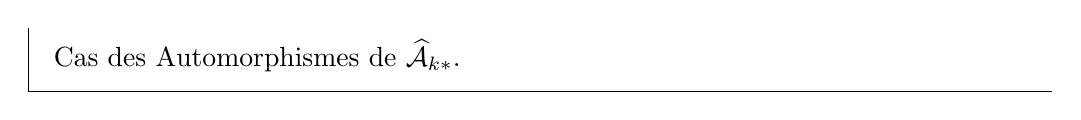
\begin{tikzpicture}
\node[anchor=west] at (.2,.45) {Cas des \uline{Automorphismes} de $\widehat{\mathcal A}_{k*}$.};
\draw (0,.8)--(0,0)--(13,0);
\end{tikzpicture}}

Nous nous intéressons maintenant aux automorphismes de la $k$-algèbre différentielle
$\tfrac12$-simpliciale $\mathcal A_{k*}=\mathcal A_*(k\{T\},k\{T\}^+,T)$.
Mais on \unsure{n'aura} de résultats simples qu'en complétant en
\[
 \widehat{\mathcal A}_{k*}\simeq(\widehat{\mathcal A}_{k,n})
\]
\[
 \begin{aligned}
 \widehat{\mathcal A}_{k,n}&\simeq k\{\{X_0,\ldots,X_n\}\}[dX_0,\ldots,dX_n]/(\textstyle\sum dX_i)\\
 &\simeq k\{\{T\}\}\{\{X_0,\ldots,X_n\}\}[dX_0,\ldots,dX_n]/
 (\textstyle\sum X_i-T,\sum dX_i)_{\mathrm{pd}}\\
 &\simeq k\{\{T\}\}\{\{X_0,\ldots,X_{n-1}\}\}[dX_0,\ldots,dX_{\unsure{n|n-1}}].
 \end{aligned}
\]

Les résultats sur les hom d'un tel $\widehat{\mathcal A}_{k,n}$ dans un
$\widehat{\mathcal A}_{k',n}$ sont les mêmes que tantôt [et peuvent s'exprimer en termes des
$\mathcal A_*(S,S^+,t)^\wedge$, (\unsure{où on fera} pour l'instant $S\simeq k\{\{T\}\}$),
avec
\[
 \mathcal A_n(S,S^+,t)^\wedge\simeq S\{\{X_0,\ldots,X_n\}\}[dX_0,\ldots,dX_n]
\]
mod idéal à p.d. engendré par $\sum X_i-t,\sum dX_i$
\[
 \simeq S\{\{X_0,\ldots,X_{n-1}\}\}[dX_0,\ldots,dX_{n-1}]\quad--
\]
mais $A'_1$ et les $B'_i$ $(i\geq1)$ sont dans
$\mathcal A_1(S,S^+,t)^\wedge\simeq S\{\{X_0\}\}$, au lieu de
$\unsure{S\{X_0\}|S\{\{X_0\}}$, i.e. les polynômes à p.d.
en $X_0$, coeff. en $S$, qui les exprimaient deviennent des séries à p.d. avec un
\margin{173}
\scanpage{175}
\begin{center}- 27 -\end{center}\hfill IX

b) Soit $n>0$ premier à l'exposant caractéristique de $k(s)$
et aux rangs des quotients des fibres géométriques de $K$ en $s$ et $t$
par leurs composantes neutres réduites, alors les deux membres de
(3.1.1) s'obtiennent en élevant $n$ respectivement à la puissance
d'exposant l'un et l'autre membre de (3.1.2), comme il résulte de la
structure connue des groupes algébriques commutatifs. Donc b) résulte de a).

c) Comme l'hypothèse $(K_{\bar t})^{\unsure{o|0}}_s$ unipotent équivaut aux relations
$\mu(t)=\alpha(t)=0$, et de même pour $K_s$, l'assertion c) résulte formellement
de b).
\figure{\begin{tikzpicture}\draw[line width=.6pt] (0,.13)--(.18,.14);\draw[line width=.6pt] (0,0)--(.18,-.02);\end{tikzpicture}}

d) L'hypothèse que $u_t$ soit une isogénie implique que $K_t$ est
fini, donc on est sous les conditions de c), et par suite $(K_{\bar s})^{\unsure{o|0}}_{\mathrm{red}}$ est
unipotent. Comme $G_s$ est de rang unipotent nul, on en déduit que $K_s$
est fini. D'ailleurs le fait que $u_t$ est une isogénie implique
$\dim G_t=\dim H_t$, et le fait que $G$ et $H$ sont plats localement de présentation finie implique $\dim G_s=\dim G_t$, $\dim H_s=\dim H_t$ (SGA 3 $\mathrm{VI_B}$ 4.3),
d'où $\dim G_s=\dim H_s$. Comme $\dim\operatorname{Ker}u_s=0$, on en conclut que
$\dim H_s=\dim u_s(G_s)$ (SGA 3 $\mathrm{VI_B}$ 1.2.), ce qui équivaut à $u_s$ plat
grâce à l'hypothèse $H_s$ lisse (SGA 3 $\mathrm{VI_A}$ 5.6). On en conclut qu'il
existe un voisinage ouvert $U$ de $s$ tel que $u$ soit plat et quasi-fini
en les points de la section unité sur $U$ (SGA 3 $\mathrm{VI_B}$ 2.2 (i) et 2.5 (ii)).
Il en résulte, comme pour $u_s$, que $u_{s'}$ est plat pour tout $s'\in U$, donc
$u|G_U$ est plat et quasi-fini, l'étant sur chaque fibre.

e) Pour la premier assertion, on se ramène aussitôt par
changement de base au cas où $S$ est intègre de point générique $t$, donc
à prouver la deuxième assertion de e). Celle-ci résulte aussitôt de d) et du
\margin{345}
\margin{345}
\margin{174}
\scanpage{176}
infinité de termes].

Soit $\varphi_*$ un \uline{\unsure{endomorphisme}} de la
$k$-algèbre diff. $\unsure{\tfrac12}$-simpliciale $\mathcal A_{k*}^\wedge$, associé à
\[
 A,\unsure{B}_i\in\widehat S_k\{\{X_0\}\}\simeq
 k\{\{T\}\}\{\{X_0\}\}\simeq k\{\{X_0,X_1\}\}
 \qquad(i\geq1)
\]
Posons
\[
 \left\{\begin{aligned}
 A&=\sum_{j\geq1}a_jX_0^{(j)}
 &&(a_j\in\widehat S_k\simeq k\{\{T\}\},j>0)\\
 \text{avec }a_j&=\sum_{h\geq0}a_{j,h}T^{(h)},
 &&a_{jh}\in k\quad\text{pour }j\geq1,h\geq0
 \end{aligned}\right.
\]
On peut aussi écrire
\[
 \left\{A=\sum_{\substack{i\geq1\\j\geq0}}\alpha_{ij}X_0^{(i)}X_1^{(j)}
 \qquad\alpha_{ij}\in k\right.
\]
Posons
\[
 \varphi_0(T)=\sum_{j\geq1}\lambda_jT^{(j)}\qquad\lambda_j\in k
\]
Ceci posé un calcul immédiat montre
\[
 \boxed{a_{1,0}=\alpha_{1,0}=\lambda_1}\quad\in k.
\]
Cet élément de $k$ s'appelle le
\deleted{\uline{indicateur}}\inserted{\deleted{discriminant}\inserted{déterminant}}
de $\varphi_*$, \inserted{noté $\Delta(\varphi_*)$}
(on peut aussi en définir si on a
$\varphi_*:\mathcal A_k^\wedge\longrightarrow \mathcal A_{k'}^\wedge$ associé à
$k\mathbin{\text{---}}k'$ donné d'avance, on trouve un élément de $k'$).

\uline{Théorème} Pour que $\varphi_*$ soit un \uline{autom.}
de $\mathcal A_{k*}^\wedge$, il f. et s. que son indicateur
soit un élément inversible de $k$. En tous cas, $\Delta(\varphi_*)$ dépend multiplicativement
de $\varphi_*$, et $\Delta(\mathrm{Id})=1$ -- donc $\Delta$ est un hom de gr.
\[
 \Omega(k)=\operatorname{Aut}_{k\,\mathrm{alg}\,\mathrm{diff}\,\unsure{\frac12\mathrm{simp}}}(\mathcal A_{k*}^\wedge)
\]
dans $k^*=G_m(k)$.
\figure{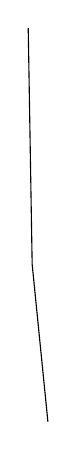
\begin{tikzpicture}\draw (0,5)--(.05,2)--(.25,0);\end{tikzpicture}}
\margin{175}
\scanpage{177}
\begin{center}- 28 -\end{center}\hfill IX

\uline{Lemme} 3.1.3. \uline{Soient} $S$ \uline{un schéma}, $K$ \uline{un} S-\uline{schéma quasi-fini}, \uline{de présentation finie}, \uline{séparé et plat sur} $S$, $s\in S$, $t\in T$ \uline{une générisation de} $s$.
\uline{Alors on a}
\[
 \operatorname{rang}K_s\leq\operatorname{rang}K_t\qquad.
\]
\uline{Si rang} $K_\eta\leq1$ \uline{pour tout point maximal de} $S$, \uline{alors}
$K\longrightarrow S$ \uline{est une immersion ouverte} (\uline{donc un isomorphisme s'il admet une section}).

Pour la première assertion, on se ramène par localisation
stricte au cas où $S$ est strictement local. Décomposant alors $K$ en
somme d'un schéma fini $K^f$ et d'un schéma à fibre spéciale vide, on
aura
\[
 \operatorname{rang}K_s=\operatorname{rang}K_s^f=\operatorname{rang}K_t^f
 \leq\operatorname{rang}K_t\qquad,
\]
la deuxième égalité provenant du fait que $K^f$ est plat, fini et de
présentation finie sur $S$, donc localement libre sur $S$.

Pour la deuxième assertion, ce qui précède montre déjà que
pour tout $s\in S$ on a $\operatorname{rang}K_s\leq1$, donc $K_s$ est vide ou isomorphe à
$\operatorname{Spec}k(s)$. Par suite $K\longrightarrow S$ est un monomorphisme (SGA 3 $\mathrm{VI_B}$ 2.11),
et étant plat et de présentation finie c'est une immersion ouverte
(EGA IV 17.9.1), ce qui achève la démonstration.

\uline{Remarque} 3.1.4. Dans 3.1 a) et la suite de la proposition 3.1, on ne
donne aucun renseignement sur ${}_nK_s$ lorsque $n$ est une puissance de $p$
(lorsque $p>1$). Lorsque $G$ est lisse (et $S$ localement noethérien ou
$H$ de présentation finie sur $S$) tout au moins, on peut donner un tel
renseignement, par essentiellement la même méthode que dans la
\figure{\begin{tikzpicture}[x=.7cm,y=.7cm]
\draw[gray] (0,.1)--(.3,.12) (.3,.5)--(.3,.15) (.5,.08)--(.7,.1)
(1.7,.1)--(1.75,.01) (2,.02)--(2.25,.15)--(2.2,.3)
(3,.1)..controls(3.3,.18)and(3.5,.08)..(3.65,.13)
(4.3,.12)--(4.55,.14)--(4.6,.05)
(5,.08)--(5.1,.05) (5.5,.06)--(5.55,.17)
(6,.05)--(6.1,.06) (6.7,.03)--(6.75,.13)
(7.5,.02)--(7.7,.13) (7.7,.03)--(8.1,.04)
(10.3,-.03)..controls(10.6,-.1)and(10.9,-.13)..(11.1,0)
(12.2,.03)--(12.5,.2) (12.6,-.06)--(12.9,-.06)
(13.3,-.1)--(13.25,.02)--(13.35,.09) (13.8,-.22)--(13.85,.4);
\end{tikzpicture}}
\margin{346}
\margin{346}
\margin{176}
\scanpage{178}
Les \deleted{\unsure{automorphismes}} éléments de $\Omega(k)$ correspondent
ainsi aux systèmes $(A,(\unsure{B_i^*|B_i})_{i\geq1})$ d'éléments
de $\widehat S_k\{\{X_0\}\}$ \deleted{\unsure{de}},
\[
 \begin{array}{l|l}
 A=\displaystyle\sum_{j\geq1}a_jX_0^{(j)}&a_j,b_{ij}\in\widehat S_k=k\{\{T\}\}\\
 B_i=\displaystyle\sum_{j\geq0}b_{ij}X_0^{(j)}&
 \end{array}
\]
tels que
\[
 \begin{aligned}
 \text{a)}\quad&\epsilon(a_1)\;(=\Delta(\varphi_*))\in k^*\\
 &(\epsilon:\widehat S_k\mathbin{\text{---}}k\text{ l'augmentation})\\
 \text{b)}\quad&2B_i=0\quad\inserted{\forall i\geq1},\quad\text{i.e. }2b_{ij}=0
 \quad\forall i\geq1,j\geq0.
 \end{aligned}
\]
On peut aussi l'écrire comme l'ens. des systèmes
$(a_{jh})_{j\geq1,h\geq0}$ $(b_{ijh})_{i\geq1,j\geq0,h\geq0}$
d'éléments de $k$ (qui \deleted{sont les coeff.} dans les
\inserted{\unsure{développements de}}\deleted{\unsure{aux}}
$a_j$ et $b_{ij}$ comme séries à p.d. en $T$) avec les seules conditions
\[
 a_{10}\in k^*,\quad 2b_{ijh}=0.
\]
Pour $k$ variable, \deleted{l'hom}\inserted{le foncteur} $\Omega(k)$ est donc
représentable par \inserted{le schéma affine sur $\mathbb Z$}
\[
 G_m\mathbin{\unsure{\times_{\mathbb Z}|\times}}
 {}_2G_{\unsure{o|a}}^{\mathbb N^*\times\mathbb N}\times_{\mathbb Z}{}_2G_a^{\mathbb N^*\times\mathbb N\times\mathbb N}
\]
\[
 \Omega\simeq\operatorname{Spec}\left(
 \mathbb Z[\deleted{\unsure{T}}(A_{jh})_{j\geq1,h\geq0},
 (B_{ijh})_{i\geq1,j\geq0,h\geq0}]
 \right.
\]
modulo idéal engendré par les $2B_{ijh}$ et localisé de plus p.r. à $A_{1,0}$

\inserted{Ainsi} $\Omega$ peut être considéré comme un schéma
en groupes sur $\mathbb Z$, qui est le schéma.
des autom. du foncteur des $\mathbb Z$-algèbres
vers les $k$-alg. différentielles $\unsure{\tfrac12}$-simpliciales
$k\longmapsto\widehat{\mathcal A}_{k*}$. (On \unsure{envisage} comme \unsure{on|mor}
\margin{177}
\scanpage{179}
\begin{center}- 29 -\end{center}\hfill IX

démonstration de a) (en se ramenant au cas $S$ local noethérien complet,
et utilisant SGA 3 XV 1.6 c), X 3.2, IX 3.6, IX 5.2), savoir :
\[
 (3.1.4.1)\qquad\operatorname{rang\,mult}({}_nK_s)\mid
 \operatorname{rang\,mult}({}_nK_t)\qquad,
\]
où rang mult désigne le rang du plus grand sous-groupe de type multiplicatif du groupe algébrique commutatif envisagé (SGA 3 XVII 7.2.1) ;
on notera qu'un groupe algébrique de type multiplicatif de torsion est
fini. La formule (3.1.4.1) est valable pour tout entier $n\geq1$. On
conclut, grâce à SGA XVII 4.6.1 (vi), que dans c), si $K_t$ est unipotent
(SGA 3 VII 1.1, il en est de même de $K_s$.

\uline{Proposition} 3.2. \uline{Soient} $S$ \uline{un schéma localement noethérien régulier
intègre de dimension} $1$, $K$ \uline{son corps des fonctions rationnelles}, $A_K$
\uline{un schéma abélien sur} $K$, $A$ \uline{son modèle de Néron sur} $S$, \uline{qui est un
schéma en groupes lisse et séparé sur} $S$ (\uline{et quasi-projectif sur} $S$
\uline{si} $S$ \uline{est noethérien} [ 23 , VIII 2, $3^\circ$]). \uline{Les conditions suivantes
sont équivalentes} :

(i) \uline{Pour tout} $s\in S$, $A_s^{\unsure{o|0}}$ \uline{est de rang unipotent nul}, \uline{i.e.}
(2.1.5) \uline{est une extension d'un schéma abélien par un tore}.

(ii) \uline{Il existe un schéma en groupes} $G$ \uline{lisse}, \uline{séparé de type
fini sur} $S$, \uline{prolongeant} $A_K$, \uline{et dont les fibres sont de rang unipotent nul}.

\uline{De plus}, \uline{si} $G$ \uline{est comme dans} (ii), \uline{alors l'unique morphisme}
$G\longrightarrow A$ \uline{induisant l'isomorphisme donné sur les fibres génériques est
un isomorphisme de} $G$ \uline{sur un sous-groupe ouvert de} $A$, \uline{donc induit un
isomorphisme des composantes neutres}
$G^{\unsure{o|0}}\xrightarrow{\sim}A^{\unsure{o|0}}$.
\margin{347}
\margin{347}
\margin{178}
\scanpage{180}
\unsure{dira|d'un}, par abus de langage, le schéma en groupe d'autom. de l'anneau différentiel
$\tfrac12$-simplicial $\widehat{\mathcal A}_{\mathbb Z*}$ --).
On a un hom de schémas en groupes
\[
 \Delta:\Omega\longrightarrow G_m
\]
et on a d'ailleurs un inverse à droite
\[
 \unsure{\delta|\sigma}:G_m\mathbin{\text{---}}\Omega
\]
($\unsure{\delta|\sigma}(\lambda)=(A,(B_i)_{i\geq1})$ avec $B_i=0\quad\forall i\geq1$,
$A=\lambda X_0$ i.e. $\varphi_1(X_0)=\lambda X_0$, d'où $\varphi_1(X_1)=\lambda X_1$,
$\varphi_0(T)=\lambda T$, $\varphi_n(X_i)=\lambda X_i\quad\forall0\leq i\leq n$.
Ainsi $\Omega$ est \deleted{\unsure{l'est}} un produit $\frac12$ direct
de $G_m$ et d'un groupe qui est (pro-)unipotent fibre par fibre
\figure{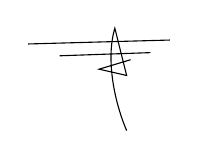
\begin{tikzpicture}
\draw (0,1.1)--(1.8,1.15) (.4,.95)--(1.55,.99);
\draw (1.25,0)..controls(1.1,.35)and(.98,.9)..(1.1,1.3)--(1.25,.7)--(.9,.78)--(1.3,.9);
\end{tikzpicture}}

Si $2$ est inversible\inserted{dans $k$}, \deleted{\unsure{dans}}
\unsure{en plus qu'en est|en plus qu'on est} \unsure{rigueur|vigueur}, tous les autom. de $\widehat{\mathcal A}_{k*}$
respectent le degré extérieur; -- donc
leur effet sur $\operatorname{Hom}(\unsure{X},\widehat{\mathcal A}_{k*})$
\inserted{$\unsure{X}$ ens. $\frac12$-simpl.}
donnent, en passant \unsure{sur la coh.}, des
opérations cohomologiques \uline{ne changeant} pas le \uline{degré} -- i.e. de degré $0$.
Donc \unsure{on ne|si on} trouve rien d'intéressant
-- \unsure{seules les op. évidentes|seules les op. cohom.} (se factorisent par $\Delta$):
\unsure{homo.th.|homoth.} par $\lambda^i$ sur $H^i$ $(\lambda\in k^*)$
\margin{179}
\scanpage{181}
\begin{center}- 30 -\end{center}\hfill IX

3.2.1. Notons tout de suite que la définition du modèle de Néron $A$
de $A_K$ est la même que dans le cas local, rappelée dans 1.1. L'existence
de ce modèle de Néron, et le fait qu'il est séparé de type fini sur $S$,
est bien connue, et se ramène en fait immédiatement au cas local.
Bien entendu, pour tout point \uline{fermé} $s\in S$, $S'=\operatorname{Spec}(O_{S,s})$ est un trait,
et $A\times_S S'$ n'est autre que le modèle de Néron de $A_K$ sur $S'$, dans le
sens envisagé dans 1.1.

Démontrons 3.2. Il est trivial que i) implique ii), car il
suffit de prendre $G=A$. Il reste donc à prouver que si $G$ est comme
dans (ii), alors $G\longrightarrow A$ est une immersion ouverte. Or c'est en effet
un cas particulier de 3.1 e).

\uline{Corollaire} 3.3. \uline{Avec les notations de} 3.2, \uline{supposons les composantes
neutres des fibres du modèle de Néron de rang unipotent nul}. \uline{Soit} $S'$
\uline{un schéma satisfaisant aux mêmes hypothèses que} $S$, $K'$ \uline{son corps des
fonctions rationnelles}, $f:S'\longrightarrow S$ \uline{un morphisme dominant},
$A_{K'}\simeq A_K\otimes_K K'\simeq$ \uline{fibre générique de} $A\times_S S'$, $A'$ \uline{le modèle de Néron de}
$A_{K'}$, \uline{et considérons le morphisme unique}
\[
 u:A\times_S S'\longrightarrow A'
\]
\uline{induisant l'identité sur les fibres génériques}. \uline{Alors} $u$ \uline{est une immersion
ouverte}, \uline{et induit donc un isomorphisme sur les composantes neutres}
\[
 (3.3.1)\qquad A^{\unsure{o|0}}\times_S S'\xrightarrow{\sim}A'^{\unsure{o|0}}\qquad.
\]

Il suffit en effet d'appliquer 3.2 dans le cas de $S'$, en
prenant $G\simeq A\times_S S'$.
\margin{348}
\margin{348}
\margin{180}
\scanpage{182}
Si donc on veut trouver des op. coh. intéressantes via les opérations de $\Omega$
\unsure{de} $\Omega(k)$ sur la coh., il faut \unsure{ess.t|en.t}
se placer \uline{en car. $2$} (\unsure{en catimini|au contraire})
-- on peut espérer trouver alors une
description des \deleted{\unsure{op.}}\inserted{\unsure{carrés}}
de Steenrod mod $2$ (regarder ce qu'il en est \unsure{en|au}).

Mais on peut essayer d'être plus astucieux, en appliquant p.ex. le foncteur
\[
 \tau_\omega:(\operatorname{Mod\,grad}S_k\Rightarrow)M\longrightarrow M_\omega
\]
donc $X_*\longmapsto\operatorname{Hom}(X_*,\mathcal A_{k*}^{\unsure{\wedge}})$ devient un
foncteur sur (Semisimpl.) à valeurs
dans les objets \inserted{algèbres} gradués diff. de $\mathcal M_\omega$
(qui est une cat. de \unsure{tenseurs} ``\unsure{de car. $k$}'',
avec $\otimes$ comm.), et on peut se
proposer, \unsure{laissant} tomber la structure
graduée au profit de la structure
d'anneau diff. sous-jacent, de
déterminer le groupe des autom.
de ce foncteur (d'abord pour $k$ fixe,
puis sa variation avec $k$). Peut-être
trouverons nous des op. coh. intéressantes
notamment puiss. de Steenrod --
\margin{\uline{Non}}
\figure{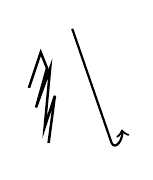
\begin{tikzpicture}
\draw[->,line width=.8pt] (0,1.6)--(.5,.15)..controls(.55,.05)and(.65,.2)..(.63,.32);
\draw[line width=.9pt] (-.55,.85)--(-.4,1.3)--(-.32,1.1)--(-.46,.6)--(-.28,1.1)--(-.35,.35)--(-.22,.75)--(-.3,.15);
\end{tikzpicture}}
\margin{181}
\scanpage{183}
\begin{center}- 31 -\end{center}\hfill IX

3.3.2. On voit donc que les propriétés équivalentes de 3.2 impliquent
une propriété de ``stabilité'' partielle pour les modèles de Néron ; on
fera attention que lorsque $A_K$ n'a pas bonne réduction i.e. que $A$ n'est
pas un schéma abélien, il n'est \uline{pas} vrai que pour tout $S'$ comme dans
3.3 (et même pour $S'$ fini sur $S$, et $K'/K$ séparable $\cdots$), le morphisme
$A\times_S S'\longrightarrow A'$ lui-même soit un isomorphisme, i.e. induise des isomorphismes
sur les groupes de composantes connexes des fibres (cf. 11.10 plus bas
pour le comportement de ces groupes de composantes connexes par extension
de la base). Ces observations, renforcées par 3.9 plus bas, justifient
la terminologie suivante, introduite par MUMFORD (et qui s'harmonise
aussi, paraît-il, avec les notions de même nom étudiées dans son livre [17]):

\uline{Définition} 3.4. \uline{Les notations étant celles de} 3.2, \uline{on dit que le schéma
abélien} $A_K$ \uline{sur} $K$ \uline{a} réduction semi-stable sur $S$ \uline{si les conditions équivalentes} (i) \uline{et} (ii) \uline{de} 3.2 \uline{sont vérifiées}.

3.4.0. On notera que sous la forme (ii), cette condition ne fait pas
appel à la notion de modèle de Néron. D'autre part, elle se ramène
immédiatement par localisation au cas où $S$ est un trait, comme il
résulte par exemple de 3.2.1. D'ailleurs, comme la formation du modèle
de Néron commute au changement de base de $S$ vers son hensélisé, ou
son hensélisé strict, la notion se ramène même au cas $S$ où $S$ est
un trait strictement local.
\margin{\unsure{345|349}}
\margin{349}
\margin{182}
\scanpage{184}
\[
 \begin{aligned}
 \mathcal A_1&=k\{X_0,X_1,dX_0,dX_1\}/(dX_0+dX_1)_{\mathrm{pd}}\\
 &=k\{T\}\{X_0,\unsure{dX_0}\}\simeq k\{T\}\{X_1,dX_1\}
 \end{aligned}
\]
\figure{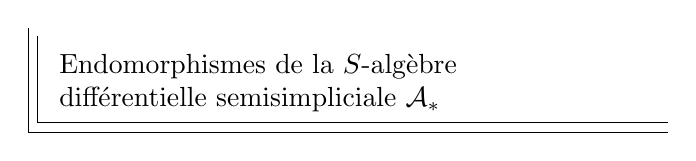
\begin{tikzpicture}
\node[anchor=west,align=left] at (.15,.5) {Endomorphismes de la $S$-algèbre\\différentielle semisimpliciale $\mathcal A_*$};
\draw (0,1.1)--(0,0)--(8,0);\draw (-.12,1.2)--(-.12,-.12)--(8,-.12);
\end{tikzpicture}}
\[
 X_0+X_1=T
\]
\[
 \varphi_1(X_0^{(i)})=\xi_i\qquad
 (1)\quad\boxed{\xi_i\xi_j=c_{ij}\xi_{i+j}}\quad i,j\geq1
\]
\margin{\deleted{$\unsure{(d\xi_1)^2=0}$}}
\[
 \varphi_1(dX_0)=d\xi_1
\]
\inserted{(il est bien de carré nul; il faut encore) et $d\xi_1$ commute aux
$\xi_i$ $(i\geq1)$ \unsure{car} $\mathcal A_1$ \uline{commut.!}}
\diagram{\[
 \begin{array}{ccc}
 \varphi_1(dX_0^{(i)})&=&d\varphi_1(X_0^{(i)})\\
 \text{''}&&\text{''}\\
 \varphi_1(X_0^{(i-1)}dX_0)&&d\xi_i\\
 \text{''}&&\\
 \xi_{i-1}d\xi_1&&
 \end{array}
\]}
\[
 (2)\quad\boxed{d\xi_i=\xi_{i-1}d\xi_1}\quad i\geq2
\]
\margin{On aura
$\varphi_1(d(X_0^{(i)}dX_0))\overset{?}{=}d\varphi_1(X_0^{(i)}dX_0)$
\deleted{$\unsure{\mathcal A_*\simeq k\cdot1}$}
\diagram{\[\begin{array}{cc}
 \text{''}&\text{''}\\
 \varphi_1(0)=0&d(\xi_i d\xi_1)\\
 &\text{''}\\&0
 \end{array}\]}}
\figure{\begin{tikzpicture}\draw[gray] (0,0)--(5.1,0)--(4.65,1.9);\end{tikzpicture}}
\diagram{\begin{tikzcd}[row sep=large]
 \mathcal A_1\arrow[d,bend right=38]\arrow[d,bend left=38,"\beta"]\\
 \mathcal A_0=k\{T\}
\end{tikzcd}}
\[
 \left\{\begin{aligned}
 \alpha(X_0^{(i)})&=0&&\forall i\geq1\\
 \alpha(dX_0)&=0
 \end{aligned}\right.
 \qquad
 \begin{aligned}
 \beta(X_0^{(i)})&=T^{(i)}&&\forall i\geq1\\
 \beta(dX_0)&=0
 \end{aligned}
\]
\[
 \left\{\begin{aligned}\alpha\circ\varphi_1&=\alpha\\\beta\circ\varphi_1&=\beta\end{aligned}\right.
\]
\[
 \begin{array}{ll}
 \alpha\circ\varphi_1(\unsure{X^{(i)}|X_0^{(i)}})=\alpha(\xi_i)&
 \text{\textcircled{3a}}\quad\boxed{\alpha(\xi_i)=0}\\
 \alpha(\unsure{X^{(i)}|X_0^{(i)}})=0&\\
 \beta\circ\varphi_1(X^{(i)})=\beta(\xi_i)&
 \text{\textcircled{3b}}\quad\boxed{\beta(\xi_i)=T^{(i)}}\\
 \beta(X^{(i)})=T^{(i)}&
 \end{array}
\]
\[
 \xi_i=\overbrace{\sum_{j\geq0}a_{ij}\deleted{\unsure{T}}X_0^{(j)}}^{A_i}
 +\overbrace{\left(\sum_{j\geq0}b_{ij}X_0^{(j)}\right)}^{B_i}dX_0
 \qquad \unsure{a_{ij}|a_j},b_{ij}\in k\{T\}
\]
(3a) s'écrit
\figure{\begin{tikzpicture}\node[draw,ellipse] {$a_{i,0}=0\quad\forall i\geq1$};\end{tikzpicture}}
\textcircled{3'a}\quad i.e.
\figure{\begin{tikzpicture}\node[draw,ellipse] {$A_i=\sum_{j\geq1}a_{ij}X_0^{(j)}$};\draw[->] (-2,.2)..controls(-2.3,.4)and(-2.45,.55)..(-2.3,.7);\end{tikzpicture}}
$\forall i\geq1$

(3b) s'écrit
\deleted{$\unsure{\sum_{j\geq1}a_{ij}X_0^{(j)}}\equiv$}
\textcircled{3'b}
\figure{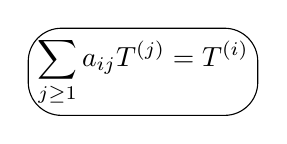
\begin{tikzpicture}\node[draw,rounded corners=12pt] {$\displaystyle\sum_{j\geq1}a_{ij}T^{(j)}=T^{(i)}$};\end{tikzpicture}}
$\forall i\geq1$
\[
 d\xi_i=\left(\sum_{j\geq1}a_{ij}X_0^{(j-1)}\right)dX_0
 =\deleted{\unsure{d\xi_i=dA_i}}
\]
\[
 d\xi_1=\left(\sum_{j\geq1}a_{1j}X_0^{(j-1)}\right)dX_0
\]
\[
 \xi_{i-1}=\sum_{j\geq1}a_{i-1,j}X_0^{(j)}
 +\left(\sum_{j\geq0}b_{i-1,j}X_0^{(j)}\right)dX_0
\]
\[
 \xi_{i-1}d\xi_1=
 \left(\sum_{k\geq1}a_{1k}X_0^{(k-1)}\right)
 \left(\sum_{\unsure{\ell}\geq1}a_{i-1,\unsure{\ell}}X_0^{(\unsure{\ell})}\right)dX_0
\]
\margin{183}
\scanpage{185}
\begin{center}- 66 -\end{center}
\hfill IX
\[
(*)\qquad v_\eta:F_\eta\longrightarrow Y_\eta\longrightarrow Y_\eta/Y_\eta^{\mathrm f}\quad .
\]
En vertu de 5.6 ce dernier groupe se prolonge en un groupe de Barsotti-Tate
ind-étale $Z$ sur $S$ (savoir $\underline M\otimes_{\mathbb Z}(Q_\ell/\mathbb Z_\ell)$). En vertu du théorème de TATE
cité dans 5.8, l'homomorphisme $(*)$ se prolonge alors en un homomorphisme
\[
v:F\longrightarrow Z\quad .
\]
Comme $F$ est à fibre spéciale connexe et que $Z$ est ind-étale, ce morphisme
est \uline{nul}. Donc il en est de même de $v_\eta$, donc $u_\eta$ se factorise par $Y_\eta^{\mathrm f}$.
C'est ce qu'il fallait démontrer !

Reste à prouver le

\uline{Lemme} 5.9.2. \uline{Soient} $S$ \uline{un trait}, $A$ \uline{un schéma en groupes néronien sur}
$S$ (1.1.2),
\[
1\longrightarrow G'\longrightarrow G\longrightarrow G''\longrightarrow 1
\]
\uline{une extension de schémas en groupes sur} $S$, \uline{avec} $G''$ \uline{lisse},
\[
u:G'\longrightarrow A
\]
\uline{un homomorphisme de groupes}, \uline{et}
\[
v_\eta:G_\eta\longrightarrow A_\eta
\]
\uline{un homomorphisme de groupes prolongeant} $u_\eta$. \uline{Supposons que l'extension}
\uline{de} $G''$ \uline{par} $A$ \uline{image de l'extension} $G$ \uline{par} $u$ \uline{soit représentable} $(*)$, - \uline{ce}
\uline{qui est le cas par exemple si} $G\longrightarrow G''$ \uline{admet une section localement}
\uline{pour la topologie} ``\uline{finie localement libre}'' (cf. SGA 3 IV 6.3) \uline{et si} $A$
\uline{est quasi-projectif sur} $S$. \uline{Alors il existe un unique morphisme de groupes}
\[
v:G\longrightarrow A
\]
\uline{prolongeant} $v_\eta$ \uline{et} $u$.

\figure{\begin{tikzpicture}\draw (0,0)--(3,0);\end{tikzpicture}}
$(*)$ Des résultats inédits de M. RAYNAUD impliquent d'ailleurs que cette
condition est toujours satisfaite.

\margin{384}
\margin{184}
\scanpage{186}
Finalement, on trouve

\uline{Proposition} Soit $S$ un anneau commutatif,
$\mathcal A_{\unsure{1}}=S\{X_0,dX_0\}$, \deleted{\unsure{on cherche à}} $S$-algèbre
diff. à puiss. divisées, avec augmentation
\[
\alpha:\mathcal A_1\mathbin{\unsure{-|\longrightarrow}}S\qquad
(\alpha(X_0^{(i)})=0\quad\forall i\geq0,\ \alpha(dX_0)=0).
\]
[\uline{NB} on regarde \unsure{bien sûr} $S$ comme anneau
différentiel à p.d. où $d_S=0$, idéal nul pour
les p.d., et $\alpha$ est compatible avec ces structures)

On cherche les endomorphismes \inserted{$\varphi$} d'\inserted{$S$-}\uline{algèbre}
\uline{différentielle} \uline{augmentée} (mais sans
p.d. !) $\varphi$ de \deleted{$\unsure{S}$} $\mathcal A$
\[
\varphi:\mathcal A\longrightarrow\mathcal A\qquad\text{endom. de $S$-algèbre}
\]
\margin{$\deleted{\varphi d\unsure{=d}}$ \inserted{\unsure{puis.}}\quad
$\varphi(x+y)=\unsure{\varphi x)|\varphi(x)}+\varphi(y)$\par
$\varphi(xy)=\varphi(x)\varphi y$\par
$\unsure{\varphi(1)|\varphi1}=1$}
\[
\varphi d=d\varphi
\qquad\qquad
\alpha\varphi=\alpha
\]
Alors $\varphi$ est donné par les
\[
\begin{array}{ccl}
\varphi(X_0^{(i)})=\xi_i\in\mathcal A&&(i\geq1)\\
\text{\textquotedbl}&&\\
A_i+B_i\,dX_0&&A_i,B_i\in S\{X_0\}\ (i\geq1)
\end{array}
\]
(on aura $\varphi(dX_0)=\deleted{\unsure{\varphi dX}}d\varphi(X_0)=d\xi_1=dA_1=\deleted{\unsure{\partial}}A'_1dX_0$)
avec les conditions
\[
\begin{cases}
A_i=A_1^{(i)}\\
\alpha(A_1)=0\quad\text{i.e.}\quad A_1\in S\{X_0\}^{+}
\end{cases}
\]
donc $\varphi$ est donné par
\[
\boxed{\boxed{\begin{cases}
A_1\in S\{X_0\}^{+}\\
B_i\in S\{X_0\}\quad(i\geq1)
\end{cases}}}
\]
sans autre condition !

Pour que $\varphi$ commute aux p.d. il f. et s.
que l'on ait
\[
\xi_i=\xi_1^{(i)}\qquad(i\geq2)
\]
ou encore
\[
B_i=A_1^{(i-1)}B_1
\]
\margin{185}
\scanpage{187}
\begin{center}- 63 -\end{center}
\hfill IX
\uline{Proposition} 5.7. \uline{Supposons} $A^{\unsure{o|0}}$ \uline{$\ell$-divisible}, $S$ \uline{hensélien}. \uline{Soit} $F_K$ \uline{un}
\uline{faisceau $\ell$-adique constructible sur} $K$ \uline{qui soit} ``\uline{non ramifié}'' \uline{i.e. qui}
\uline{se prolonge en un faisceau $\ell$-adique constant tordu} $F$ \uline{sur} $S$, \uline{et soit}
$u:F_K\longrightarrow T_\ell(A_K)$ \uline{un homomorphisme de pro-groupes}, \uline{alors} $u$ \uline{se factorise}
\uline{en un homomorphisme de} $F$ \uline{dans} $T_\ell(A_K)^{\mathrm f}$.

En effet, on aura
\[
(5.7.1)\qquad u=(u(\nu))_{\nu\geq0},\quad\text{avec }u(\nu):F_K(\nu)\longrightarrow T_\ell(A_K)(\nu)={}_{\ell^\nu}A_K\quad .
\]
Par la propriété universelle de $A$, comme $F(\nu)$ est étale donc lisse sur
$S$, le morphisme $u(\nu)$ provient d'un homomorphisme
\[
v(\nu):F(\nu)\longrightarrow{}_{\ell^\nu}A\quad ,
\]
et par définition de la partie fixe, cet homomorphisme se factorise en
\[
v(\nu):F(\nu)\longrightarrow({}_{\ell^\nu}A)^{\mathrm f}\quad .
\]
Comme l'image du morphisme induit sur les fibres spéciales tombe dans
la partie infiniment $\ell$-divisible de $A_{\unsure{o|0}}$, on conclut que $v(\nu)$ se factorise
même par $({}_{\ell^\nu}A^{\unsure{o|0}})^{\mathrm f}$. Par passage à la limite sur $\nu$, on trouve un homomorphisme
\[
v:F\longrightarrow T_\ell(A^{\unsure{o|0}})^{\mathrm f}\quad ,
\]
et le morphisme induit sur les fibres génériques donne évidemment la
factorisation cherchée.

\uline{Remarques} 5.7.2. Lorsque $\ell\ne p$, il est clair que la propriété 5.7 du
sous-pro-groupe $T_\ell(A_K)^{\mathrm f}$ de $T_\ell(A_K)$ caractérise celui-ci de façon unique,
comme le plus grand sous-faisceau $\ell$-adique de $T_\ell(A_K)$ qui soit ``non ramifié''.
Lorsque $\ell=p$, l'énoncé 5.7 cesse d'être bien raisonnable, et on va donner

\margin{381}
\margin{381}
\margin{186}
\scanpage{188}
Donc ces $\varphi$ correspondent exactement aux
\[
\xi_1\deleted{{}=A_1+B_1dX_0}\ \in\operatorname{Ker}\alpha=\mathcal A^+
\]
i.e. \deleted{\unsure{aux}} (posons $\xi_1=A_1+B_1dX_0$, $A_1,B_1\in\unsure{B|S}\{X_0\}$)
aux couples
\[
A_1\in S\{X_0\}^{+},\quad B_1\in S\{X_0\}
\]

\figure{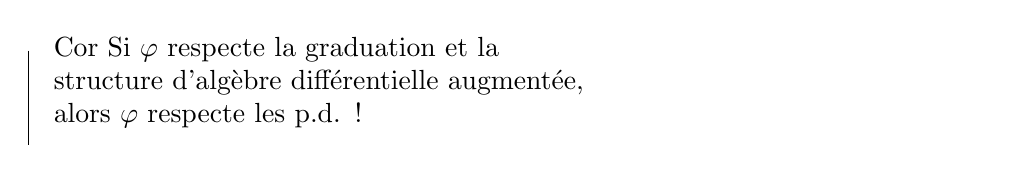
\begin{tikzpicture}
\draw (0,0)--(0,-1.2);
\node[anchor=north west,text width=12cm] at (.2,.3) {\uline{Cor} Si $\varphi$ respecte la graduation \uline{et} la\\
structure d'algèbre différentielle augmentée,\\
alors $\varphi$ respecte les p.d. !};
\end{tikzpicture}}

On prend maintenant $S=k\{T\}$, et
on regarde $S$ comme muni d'un idéal à
p.d. \deleted{\unsure{0}}\inserted{$k\{T\}^{+}$} pour $\mathcal A=\mathcal A_1$. Donc $\alpha$ est
compatible avec toutes ces structures, y
compris les p.d. On définit
\[
\begin{array}{rcll}
\beta:\mathcal A_1&=S\{X_0,dX_0\}=k\{T\}\{X_0,dX_0\}&\longrightarrow&S\\
&\simeq S\{X_0,X_1,dX_0,dX_1\}/(X_0+X_1-T,dX_0+dX_1)_{\mathrm{pd}}&&\text{\textquotedbl}\\
&&&k\{T\}
\end{array}
\]
par la condition que $\beta$ est comp. avec
toutes les structures, et
\margin{\figure{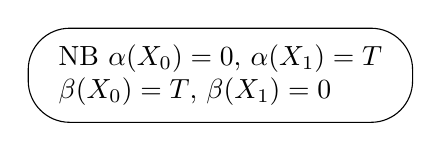
\begin{tikzpicture}
\node[draw,rounded corners=15pt,inner sep=5pt] {\begin{tabular}{ll}NB $\alpha(X_0)=0$, $\alpha(X_1)=T$\\
$\beta(X_0)=T$, $\beta(X_1)=0$\end{tabular}};
\end{tikzpicture}}}
\[
\beta(X_0)=T\qquad\text{donc}\quad
\begin{cases}\beta(X_0^{(i)})=T^{(i)}\\\beta(dX_0)=0\end{cases}
\]
et on s'intéresse aux $\varphi$ \inserted{(un hom. d'alg. diff. sur $S$)} compatibles
avec l'augmentation $\alpha$ \uline{et} $\beta$, Cela
signifie que l'on a $\beta\varphi=\beta$ i.e.
\[
\beta\underbrace{\varphi(X_0^{(i)})}_{A_1^{(i)}+B_i\,dX_0}
=\deleted{\unsure{\xi_1}}\beta(X_0^{(i)})\quad\text{pour }\forall i\geq1,\quad\text{ou encore}
\]
\[
\beta(A_1)^{(i)}=T^{(i)}\qquad\forall i\geq1\qquad\text{ou encore}
\]
\margin{187}
